\documentclass[11pt]{article}
\usepackage[margin=1.05in]{geometry}
\usepackage[T1]{fontenc}
\usepackage{lmodern,microtype}
\usepackage{amsmath,amssymb,amsthm,mathtools}
\usepackage{booktabs,graphicx,enumitem,xcolor}
\usepackage[hidelinks]{hyperref}
\usepackage{url}
\usepackage[nameinlink,noabbrev]{cleveref}
\setlist{nosep,leftmargin=1.6em}
\setlength{\parskip}{3pt}
\renewcommand{\arraystretch}{1.08}
\setlength{\tabcolsep}{3.5pt}

\newtheorem{theorem}{Theorem}[section]
\newtheorem{lemma}[theorem]{Lemma}
\newtheorem{proposition}[theorem]{Proposition}
\newtheorem{corollary}[theorem]{Corollary}
\theoremstyle{definition}
\newtheorem{definition}[theorem]{Definition}
\newtheorem{assumption}[theorem]{Assumption}
\newtheorem{example}[theorem]{Example}
\theoremstyle{remark}
\newtheorem{remark}[theorem]{Remark}
\newtheorem{conjecture}[theorem]{Conjecture}

\newcommand{\E}{\mathbb{E}}
\newcommand{\Var}{\operatorname{Var}}
\newcommand{\Cov}{\operatorname{Cov}}
\newcommand{\R}{\mathbb{R}}
\newcommand{\one}{\mathbf{1}}
\newcommand{\tr}{\operatorname{tr}}
\newcommand{\ind}{\mathbb{1}}
\DeclareMathOperator*{\argmax}{arg\,max}
\newcommand{\EoneMinRho}{0.8536}
\newcommand{\EfiveIntKS}{0.047}
\newcommand{\EfiveSE}{0.200}
\newcommand{\EfourOncePred}{1.1450}
\newcommand{\EfourOnceSim}{1.1445$\pm$0.0013}
\newcommand{\EfourFA}{0.180}
\newcommand{\EfourNJc}{0.0042}
\newcommand{\EfourNJs}{0.0041}
\newcommand{\EfiveProbeA}{4.5}
\newcommand{\EfiveProbeB}{1.75}

\usepackage{environ}
\NewEnviron{expsec}{\global\let\expbody\BODY}

\title{Estimation Robustness of Static Congestion Pricing under Learned Demand}
\author{Shereen Anand\thanks{The author is currently affiliated with Microsoft Research. This research was conducted independently of her work at Microsoft Research.}\\Independent Researcher\\\texttt{pes1202201328@pesu.pes.edu}}
\date{}

\begin{document}
\maketitle

\begin{abstract}
Congestion-pricing deployments often use simple, mostly static tolls. Recent work shows that with known demand, the revenue loss from doing so is bounded in canonical traffic models, but these guarantees assume the planner knows demand. In practice, demand is estimated from traffic that the toll itself shapes. We study whether simple tolls retain their guarantees under learned demand in a two-period congestion model with linear demand response and several extensions. The objective loss of any plug-in tolling policy is an \emph{exact} quadratic form in toll error (Lemma~\ref{lem:quad}), yielding the following results. (i) With known demand, the two-period price of simplicity is tight at $(1+\sqrt2)/(2\sqrt2)\approx0.854$, attained at demand ratio $1+\sqrt2$; with $H$ periods no constant guarantee holds, since the worst-case ratio decays like $4/H_H$ (Theorems~\ref{thm:known} and~\ref{thm:generalH}). (ii) Estimation error increases the dynamic plug-in's loss relative to its dynamic oracle by at least as much as it increases the static plug-in's loss relative to its static oracle. The dynamic plug-in outperforms the static plug-in exactly when the true toll differential exceeds the root-mean-square error of the estimated differential (Corollary~\ref{cor:cross}); the loss ordering extends to periods coupled by cross-period substitution (Theorem~\ref{thm:coupled}). (iii) This simplicity advantage applies to \emph{unshrunk} plug-in estimators: certainty equivalence is Bayes-optimal in the interior regime, so a Bayesian dynamic planner weakly dominates a Bayesian static planner (Theorem~\ref{thm:bayes}), and a one-parameter shrinkage family interpolates between them with closed-form risk (Theorem~\ref{thm:shrink}). (iv) The static-optimal toll is identifiable from aggregate flows under one fixed toll, while the dynamic-optimal toll is not identifiable under any interior toll sequence (Propositions~\ref{prop:ident-static}--\ref{prop:ident-split}). (v) Under random-walk demand, batched re-estimation has an interior optimal review period; a continuously updated Kalman filter strictly dominates every batched schedule even with revision costs, and a one-time estimate never recovers from a demand shift (Theorems~\ref{thm:review} and~\ref{thm:kalman}). We verify closed forms with seeded CPU simulations and report discrepancies.
\end{abstract}

\section{Introduction}\label{sec:intro}
Congestion-pricing systems often use simple, mostly static tolls, while few deploy optimal time-varying prices. Jalota, Di and Elmachtoub~\cite{jde2026} recently quantified what simplicity costs when demand is known. In Vickrey's bottleneck model with a public-transit outside option and in a city-scale Macroscopic Fundamental Diagram (MFD) model, they show that revenue-optimal static tolls achieve a constant fraction of the optimal dynamic revenue (at least two thirds across many practically relevant regimes in the current arXiv version) and at most twice the minimum achievable system cost.

The guarantee has a quiet premise: the planner knows demand. A real planner does not. Demand must be estimated from observed traffic, and the toll in place changes the traffic that is observed: drivers priced off the road leave no trace in the counts. Learning and pricing are therefore coupled, and it is not obvious that a rule which is near-optimal under perfect information remains so when its inputs are estimated. It is equally unclear whether more adaptive pricing helps, since an adaptive rule must estimate \emph{more}, from data its own past decisions have distorted.

This paper studies the price of simplicity under learned demand in the smallest model in which the question is well posed: $H$ periods per day (mostly $H=2$, peak and off-peak), linear demand response, a linear congestion externality, and a planner who observes noisy flows. The model is deliberately reduced-form. It isolates the statistical structure of the problem while sacrificing the departure-time richness of the bottleneck model. Within it every quantity of interest is computable in closed form, and the answers are sharper than one might expect.

\paragraph{Contributions.}
\begin{enumerate}
\item \textbf{Known demand (Section~\ref{sec:known}).} The revenue ratio between the optimal static and optimal dynamic toll for two periods is at least $(1+\sqrt2)/(2\sqrt2)\approx0.854$, with equality at demand ratio $1+\sqrt2$ (Theorem~\ref{thm:known}). With $H$ periods the ratio is bounded below by $4mM/(m+M)^2$ in terms of the extreme period demands, and this dependence is unavoidable: on a power-law profile it decays like $4/H_H$ (Theorem~\ref{thm:generalH}).
\item \textbf{Estimated demand (Section~\ref{sec:est}).} Estimation error is not neutral between policy classes. The plug-in dynamic toll loses exactly $\lambda\sum_i(u_i-\bar u)^2$ more than the plug-in static toll, in toll-error units, for either the revenue or the welfare objective (Theorem~\ref{thm:est}). The statement survives, verbatim in a suitable metric, when periods are coupled by cross-period substitution (Theorem~\ref{thm:coupled}), a reduced model of schedule shifting that was left as a conjecture in an earlier version of this work.
\item \textbf{Beyond plug-in (Section~\ref{sec:bayes}).} Certainty equivalence is Bayes-optimal under quadratic loss (Theorem~\ref{thm:bayes}). Shrinkage interpolates between static and dynamic tolls with a closed-form optimal weight, while James--Stein shrinkage dominates the dynamic plug-in for $H\ge4$ (Theorem~\ref{thm:shrink}).
\item \textbf{Identifiability (Section~\ref{sec:ident}).} The static-optimal toll is identified from aggregate counts under a single fixed toll; the split of demand across periods, hence the dynamic-optimal toll, is not identified from aggregate counts under any toll sequence that keeps all periods active. Corner probes reveal it at an explicit revenue cost.
\item \textbf{Learning dynamics (Section~\ref{sec:dyn}).} Under random-walk demand there is an interior optimal review period in the class of batched cycle-mean policies (Theorem~\ref{thm:review}); daily batching is optimal exactly when $\sigma^2/\nu^2\le3/2$. A Kalman filter beats the whole batched class, \emph{also} when revisions are costly (Theorem~\ref{thm:kalman}); the matched-gain EWMA is exactly the steady-state Kalman filter. Deterministic drift obeys a cube-root law (Proposition~\ref{prop:drift}) and a one-time estimate never recovers from a demand shift (Proposition~\ref{prop:recovery}).
\item \textbf{Simulation evidence (Appendix~\ref{sec:exp}).} We pair every closed form with a simulation and test ablations on error structure, demand dynamics, change-point detection, unknown slope, boundary effects, period count and heteroskedasticity. We report deviations when the interior approximation fails.
\end{enumerate}
For clarity, Theorem~\ref{thm:est} compares the static plug-in toll with the static oracle and the dynamic plug-in toll with the dynamic oracle; part~(d) gives the cross-class comparison between the two plug-in policies.

\paragraph{Scope.} Everything proved is elementary and proved in full (Appendix~\ref{app:proofs}). The extensions to Vickrey's bottleneck model and to the MFD model are stated as open conjectures and are \emph{not} claimed.

\section{Model}\label{sec:model}
\subsection{Setup}
Time is indexed by days $t=1,2,\dots$; each day has $H$ periods $i\in\{1,\dots,H\}$ ($H=2$ unless stated). In period $i$ of day $t$ there is a potential demand $a_{i,t}>0$: the mass of users who would consider the road. Users' values are distributed so that demand at generalized price $p$ is linear,
$x_i=a_{i,t}-bp$ whenever $0\le x_i\le a_{i,t}$, with price sensitivity $b>0$; equivalently the inverse value function is $v_i(x)=(a_{i,t}-x)/b$. Using the road in period $i$ imposes a congestion cost $cx_i$ on each of its $x_i$ users ($c>0$), so the generalized price under toll $\tau_i$ is $p_i=\tau_i+cx_i$. Solving the fixed point $x_i=a_{i,t}-b(\tau_i+cx_i)$ gives, in the interior,
\begin{equation}\label{eq:usage}
x_i(\tau_i)=\frac{a_{i,t}-b\tau_i}{1+bc}=\alpha_{i,t}-\beta\tau_i,\qquad \alpha_{i,t}:=\frac{a_{i,t}}{1+bc},\quad\beta:=\frac{b}{1+bc}.
\end{equation}
Here $\alpha_{i,t}$ is usage at zero toll and $\beta$ is the toll sensitivity of usage. We work in $(\alpha,\beta)$ coordinates for revenue and in $(a,b,c)$ coordinates for welfare. Outside the interior regime usage is clipped, $x_i=\max(\alpha_i-\beta\tau_i,0)$.

\subsection{Objectives and toll classes}
The planner's objective is either toll revenue $R(\tau)=\sum_i\tau_ix_i(\tau_i)$ or social welfare $W(\tau)=\sum_i\big[\int_0^{x_i}v_i(z)\,dz-cx_i^2\big]$ (tolls are transfers and cancel). Both are concave quadratics in $\tau$ in the interior regime.

\begin{definition}[Toll classes]\label{def:classes}
A \emph{dynamic} policy chooses $(\tau_1,\dots,\tau_H)$ freely. A \emph{static} policy is restricted to $\tau_1=\dots=\tau_H$. Across days, an \emph{estimate-once} policy forms one demand estimate and fixes its toll; an \emph{$m$-scheduled} policy re-estimates every $m$ days and holds the toll between reviews; a \emph{continuous} policy re-estimates daily ($m=1$). Within a class the planner uses \emph{plug-in} (certainty-equivalent) tolls: the toll that would be optimal if the current estimate were exact.
\end{definition}

\begin{definition}[Observation models]\label{def:obs}
After tolls are set on day $t$ the planner observes flows with independent mean-zero noise of variance $\sigma^2$. (O1) \emph{Aggregate flow}: only $Y_t=\sum_ix_{i,t}+\xi_t$ is observed (e.g.\ counts at a bottleneck exit). (O2) \emph{Per-period flows}: $Y_{i,t}=x_{i,t}+\xi_{i,t}$ for each period. The planner knows $b$ and $c$ (hence $\beta$) and not the demand levels; Proposition~\ref{prop:slope} relaxes known $\beta$.
\end{definition}

\begin{assumption}[Interior regime]\label{ass:interior}
At all tolls considered usage is interior, $0<x_i<a_i$. For known-demand results this requires a demand ratio below $3$ (Section~\ref{sec:known}); for estimation results it requires errors small relative to demand. Corner behaviour is analysed where it changes conclusions (Theorems~\ref{thm:known}, \ref{thm:generalH}) and is otherwise quantified in the ablations of Section~\ref{sec:exp}.
\end{assumption}

\subsection{What the model is and is not}
The model is a reduced form of the bottleneck-with-transit framework of~\cite{jde2026}: the congestion externality $cx_i$ stands in for queueing delay, the linear value distribution stands in for the transit outside option and scheduling preferences, and the periods stand in for the within-day time profile. It captures the revenue and welfare geometry of the pricing problem and the statistical coupling between tolls and observations. It does not capture departure-time substitution except through the reduced cross-period coupling of Section~\ref{sec:coupled}. Section~\ref{sec:open} states what we conjecture carries over.

\section{The price of simplicity with known demand}\label{sec:known}
All proofs are in Appendix~\ref{app:proofs}.

\begin{lemma}[Exact quadratic losses]\label{lem:quad}
In the interior regime:\\
(a) \emph{Revenue.} The optimal dynamic tolls are $\tau^D_i(\alpha)=\alpha_i/(2\beta)$ and the loss from any toll vector $\tau$ is exactly
\[R^D(\alpha)-R(\tau;\alpha)=\beta\sum_{i}\Big(\tau_i-\frac{\alpha_i}{2\beta}\Big)^2.\]
(b) \emph{Welfare.} The optimal dynamic tolls are the Pigouvian tolls $\tau^W_i(a)=a_ic/(1+2bc)$ and
\[W^D(a)-W(\tau;a)=\lambda\sum_i\Big(\tau_i-\frac{a_ic}{1+2bc}\Big)^2,\qquad \lambda:=\frac{b(1+2bc)}{2(1+bc)^2}.\]
\end{lemma}
Lemma~\ref{lem:quad} is the engine of the paper: because the loss is an exact squared distance to the optimal toll, every question about policy classes becomes a question about projections onto the static subspace $\{\tau_1=\dots=\tau_H\}$, and every question about estimation becomes a question about squared errors.

\begin{theorem}[Price of simplicity, known demand, $H=2$]\label{thm:known}
Let $r:=\max_i\alpha_i/\min_i\alpha_i\ge1$. The revenue ratio of the optimal static to the optimal dynamic toll is
\[\rho(\alpha)=\frac{R^S(\alpha)}{R^D(\alpha)}=\begin{cases}\dfrac{(\alpha_1+\alpha_2)^2}{2(\alpha_1^2+\alpha_2^2)},&1\le r\le1+\sqrt2,\\[8pt]\dfrac{r^2}{1+r^2},&r\ge1+\sqrt2,\end{cases}\]
which satisfies $\rho(\alpha)\ge\frac{1+\sqrt2}{2\sqrt2}=\frac12+\frac1{2\sqrt2}\approx0.8536$, with equality exactly at $r=1+\sqrt2$. Moreover $\rho=1$ iff $\alpha_1=\alpha_2$, and $\rho\to1$ as $r\to\infty$.
\end{theorem}

\begin{remark}\label{rem:corner}
The worst case is not extreme asymmetry: beyond $r=1+\sqrt2\approx2.41$ the optimal static toll prices out the small period entirely, and since the dynamic optimum collects relatively little there, the ratio recovers. The interior formula alone would suggest a worst case of $1/2$; accounting for the non-negativity of usage lifts the true worst case to $0.8536$. This sits comfortably above the two-thirds guarantee that~\cite{jde2026} prove for their models. The two models differ, and nothing here bears on the worst-case constant in the bottleneck model.
\end{remark}

\subsection{More than two periods}
With $H$ periods the interior-regime ratio is $(\sum_i\alpha_i)^2/(H\sum_i\alpha_i^2)$, and the corner analysis of Theorem~\ref{thm:known} does not generalise in closed form. The following result gives a clean lower bound that holds without any interior assumption, and shows that it cannot be improved to a constant.

\begin{theorem}[General $H$: bounded heterogeneity is necessary and sufficient]\label{thm:generalH}
Let $\alpha\in\R^H_{>0}$ with $m=\min_i\alpha_i$ and $M=\max_i\alpha_i$.\\
(a) For every $\alpha$ (with or without binding corners),
\[\rho(\alpha)\ \ge\ \frac{(\sum_i\alpha_i)^2}{H\sum_i\alpha_i^2}\ \ge\ \frac{4mM}{(m+M)^2}.\]
(b) For the power-law profile $\alpha^{(H)}_i=\sqrt{H/i}$, $i=1,\dots,H$,
\[\rho\big(\alpha^{(H)}\big)\ \le\ \frac{4}{H_H},\qquad H_H=\sum_{i=1}^H\frac1i,\]
so that $\inf_{H,\alpha}\rho(\alpha)=0$: no constant guarantee holds in this reduced model for arbitrary profiles as $H$ grows (the bound is informative once $H_H>4$).
\end{theorem}
Part (a) is the interior Kantorovich-type bound; we do not claim it is tight once corners bind. For $H=2$ it is dominated by Theorem~\ref{thm:known}. Part (b) says constant-factor guarantees such as those of~\cite{jde2026} cannot be a property of the reduced linear model alone: they rely on structure of the bottleneck and MFD models that bounds how heterogeneous the effective period demands can be.

\section{Estimated demand: simplicity is robustness}\label{sec:est}
With demand unknown, the planner forms estimates $\hat\theta=\theta+\varepsilon$ and sets plug-in tolls. Write $u_i:=\tau^*_i(\hat\theta)-\tau^*_i(\theta)$ for the resulting error in toll units (for revenue $u_i=\varepsilon_i/(2\beta)$ where $\varepsilon_i$ is the error in $\hat\alpha_i$; for welfare $u_i=c\varepsilon_i/(1+2bc)$ where $\varepsilon_i$ is the error in $\hat a_i$).

\begin{theorem}[Estimation error hurts flexible tolls more]\label{thm:est}
Consider any objective satisfying Lemma~\ref{lem:quad} with curvature $\lambda>0$ and optimal-toll map affine in the demand parameters, over $H$ periods, in the interior regime. Let $G:=\lambda\sum_i(\tau^*_i(\theta)-\bar\tau^*(\theta))^2$ be the known-demand gap between the optimal dynamic and optimal static toll, and $u\in\R^H$ the toll error of a plug-in estimator. Then:
\begin{enumerate}[label=(\alph*)]
\item $L^D(\varepsilon):=\mathrm{Obj}^D(\theta)-\mathrm{Obj}(\tau^*(\hat\theta);\theta)=\lambda\|u\|^2$;
\item $L^S(\varepsilon):=\mathrm{Obj}^S(\theta)-\mathrm{Obj}(\bar\tau^*(\hat\theta)\one;\theta)=\lambda H\bar u^2$, the excess over the static oracle, where $\bar u=\frac1H\sum_iu_i$;
\item hence $L^D-L^S=\lambda\sum_i(u_i-\bar u)^2\ge0$, with equality iff all $u_i$ are equal;
\item the realized advantage of the dynamic plug-in over the static plug-in is $G-\lambda\sum_i(u_i-\bar u)^2$.
\end{enumerate}
\end{theorem}
Each policy's loss is measured against its own class's oracle; the cross-class comparison is (d). The static plug-in pays only for the error in the average optimal toll, the dynamic plug-in pays for the whole error vector.

\begin{corollary}[Revenue specialization]\label{cor:rev}
For the revenue objective with $H=2$ and errors $\varepsilon_i$ in $\hat\alpha_i$: $L^S=(\varepsilon_1+\varepsilon_2)^2/(8\beta)$, $L^D=(\varepsilon_1^2+\varepsilon_2^2)/(4\beta)$, $L^D-L^S=(\varepsilon_1-\varepsilon_2)^2/(8\beta)\ge0$ and $G=(\alpha_1-\alpha_2)^2/(8\beta)$. If $\varepsilon_1,\varepsilon_2$ are i.i.d.\ with variance $\sigma_\alpha^2$ then $\E L^S=\sigma_\alpha^2/(4\beta)$ and $\E L^D=\sigma_\alpha^2/(2\beta)$: the dynamic rule loses twice as much revenue to estimation error.
\end{corollary}

\begin{corollary}[Welfare specialization]\label{cor:welf}
For the welfare objective with $H=2$ and errors $\varepsilon_i$ in $\hat a_i$ the same conclusions hold with $\kappa:=bc^2/\big(4(1+bc)^2(1+2bc)\big)$ in place of $1/(8\beta)$: $L^S=\kappa(\varepsilon_1+\varepsilon_2)^2$, $L^D=2\kappa(\varepsilon_1^2+\varepsilon_2^2)$, $L^D-L^S=\kappa(\varepsilon_1-\varepsilon_2)^2$, $G=\kappa(a_1-a_2)^2$.
\end{corollary}

\begin{corollary}[When the simple toll wins]\label{cor:cross}
The expected realized advantage of the dynamic plug-in over the static plug-in is $G-\lambda\E\sum_i(u_i-\bar u)^2$. For $H=2$,
\[\text{dynamic wins in expectation}\iff\E\big[(u_1-u_2)^2\big]<\big(\tau^*_1(\theta)-\tau^*_2(\theta)\big)^2,\]
i.e.\ exactly when the true optimal-toll differential exceeds the root-mean-square error of the estimated differential. For revenue with i.i.d.\ errors this reads $\sigma_\alpha^2<(\alpha_1-\alpha_2)^2/2$. No centering assumption on the errors is needed: bias and variance enter symmetrically through $\E[(u_1-u_2)^2]$.
\end{corollary}

\begin{remark}[Correlated errors, bias, heavy tails]\label{rem:corr}
For centered errors the static advantage is $(\lambda/2)\Var(u_1-u_2)=\lambda\sigma_u^2(1-\varrho)$ when $\Var(u_i)=\sigma_u^2$ and $\mathrm{corr}(u_1,u_2)=\varrho$. Perfectly correlated (common-mode) errors give equality, not a dynamic advantage: $u_1=u_2$ a.s.\ implies $L^D=L^S$. Anti-correlated errors maximise the static advantage. A common-mode bias leaves $L^D-L^S$ unchanged, a differential bias $b_1-b_2$ adds $\lambda(b_1-b_2)^2/2$. The common-mode case is the realistic worry (a shared demand shock misread in both periods) and is the boundary at which the theorem stops helping the simple toll; it never reverses the inequality. Tail weight does not enter at the level of expectations, but heavy tails drive plug-in tolls into the corner regime where Lemma~\ref{lem:quad} fails (Section~\ref{sec:exp}, ablation A2).
\end{remark}

\begin{remark}[A caveat on the reach of the result]\label{rem:caveat}
If the demand split is known from historical data and only the level is uncertain, the dynamic rule's estimation burden largely disappears and Corollary~\ref{cor:cross} favours it. The theorem compares policy classes given \emph{symmetric} uncertainty about the period demands. Section~\ref{sec:bayes} sharpens this: the correct reading is that naive flexibility is fragile, not that flexibility is.
\end{remark}

\subsection{Periods coupled by cross-period substitution}\label{sec:coupled}
In the bottleneck model a toll in one period shifts departures to neighbouring periods. A minimal reduced form of this is a linear demand system with cross effects,
\begin{equation}\label{eq:coupled}
x=\alpha-B\tau,\qquad B=B^\top\succ0,
\end{equation}
e.g.\ $B=\beta I+\kappa\mathcal L$ with $\mathcal L$ the Laplacian of the path graph on periods, in which a higher toll in period $i$ moves users to periods $i\pm1$ (strength $\kappa$). Revenue is $R(\tau;\alpha)=\tau^\top(\alpha-B\tau)$.

\begin{theorem}[Coupled periods]\label{thm:coupled}
Under \eqref{eq:coupled} in the interior regime, let $\langle y,z\rangle_B=y^\top Bz$ and let $P$ be the $B$-orthogonal projector onto $\mathrm{span}(\one)$, $Py=\frac{\one^\top By}{\one^\top B\one}\one$. Then:
\begin{enumerate}[label=(\alph*)]
\item $\tau^D=\tfrac12B^{-1}\alpha$, $R^D=\tfrac14\alpha^\top B^{-1}\alpha$, and $R^D-R(\tau)=\|\tau-\tau^D\|_B^2$.
\item The static optimum is $c^S=\one^\top\alpha/(2\,\one^\top B\one)$ with $R^S=(\one^\top\alpha)^2/(4\,\one^\top B\one)$, and $R^S-R(c\one)=(\one^\top B\one)(c-c^S)^2$.
\item For plug-in tolls built from $\hat\alpha=\alpha+\varepsilon$, with $u:=\tfrac12B^{-1}\varepsilon$ the toll error,
\[L^D=\|u\|_B^2=\tfrac14\varepsilon^\top B^{-1}\varepsilon,\qquad L^S=\|Pu\|_B^2=\frac{(\one^\top\varepsilon)^2}{4\,\one^\top B\one},\qquad L^D-L^S=\|(I-P)u\|_B^2\ge0,\]
with equality iff $\varepsilon\propto B\one$.
\item The realized advantage of the dynamic plug-in is $G-\|(I-P)u\|_B^2$ with $G=\|(I-P)\tau^D\|_B^2=R^D-R^S$. For $\E\varepsilon=0$, $\Cov\varepsilon=\Sigma$, the dynamic plug-in wins in expectation iff
\[G>\tfrac14\Big[\tr(B^{-1}\Sigma)-\frac{\one^\top\Sigma\one}{\one^\top B\one}\Big].\]
\end{enumerate}
\end{theorem}
For $B=\beta I$ this is Theorem~\ref{thm:est}. The ordering ``estimation error hurts the flexible toll at least as much'' therefore survives cross-period substitution exactly, in the $B$-metric. What it does \emph{not} do is settle the bottleneck model, where the demand map is not linear in the toll; Conjecture~\ref{conj:bottle} remains open.

\section{Beyond plug-in: Bayes, shrinkage, and what simplicity is really robust to}\label{sec:bayes}
The statement ``fewer estimated parameters beat more under noise'' is a bias--variance statement, and bias--variance statements are statements about an estimator class. Here the estimator is the unshrunk plug-in. Two results make the statement precise.

\begin{theorem}[Certainty equivalence is Bayes-optimal; flexibility has non-negative value]\label{thm:bayes}
Let the objective satisfy $\mathrm{Obj}(\tau;\theta)=\mathrm{Obj}^D(\theta)-\lambda\|\tau-\tau^*(\theta)\|^2$ with $\tau^*$ affine in $\theta$, and let $\pi$ be a posterior for $\theta$ with finite second moments, $\bar\theta=\E_\pi\theta$. For any linear toll class $\mathcal T\subseteq\R^H$ with Euclidean projector $\Pi_{\mathcal T}$:
\begin{enumerate}[label=(\roman*)]
\item the unique posterior-expected-objective maximiser in $\mathcal T$ is $\Pi_{\mathcal T}\,\tau^*(\bar\theta)$: plug in the posterior mean, then project (average, for the static class);
\item its posterior expected loss against the dynamic oracle is $\lambda\big[\tr\Cov_\pi(\tau^*)+\|(I-\Pi_{\mathcal T})\tau^*(\bar\theta)\|^2\big]$;
\item consequently the posterior value of flexibility is $V=\lambda\|(I-\Pi_{\rm static})\tau^*(\bar\theta)\|^2\ge0$, that is, under Bayes-optimal estimation the dynamic class weakly dominates the static class for every posterior.
\end{enumerate}
\end{theorem}

Part (iii) does not contradict Theorem~\ref{thm:est}: there the dynamic planner uses the \emph{unshrunk} estimate $\tau^*(\hat\theta)$, whose differential $(I-P)\hat\tau$ is inflated by noise, while the Bayes-optimal dynamic planner uses the posterior mean, which shrinks the differential toward what the prior supports. Corollary~\ref{cor:cross} is therefore exactly a statement about naive flexibility.

Exchangeable Gaussian priors make this quantitative. Suppose a planner observes toll-space estimates $\hat\tau_i=\tau^*_i+u_i$ with $u_i$ i.i.d.\ mean zero variance $s^2$ (this covers (O2) with $u_i=\varepsilon_i/(2\beta)$), and write $d_i=\tau^*_i-\bar\tau^*$, $D=\sum_id_i^2$. Consider the family
\begin{equation}\label{eq:shrink}
\hat\tau(w)=\bar{\hat\tau}\,\one+w\,(\hat\tau-\bar{\hat\tau}\one),\qquad w\in[0,1],
\end{equation}
which is static at $w=0$ and the dynamic plug-in at $w=1$.

\begin{theorem}[Interpolating between static and dynamic]\label{thm:shrink}
(a) The expected toll-space loss $\E\|\hat\tau(w)-\tau^*\|^2$ equals $s^2+w^2(H-1)s^2+(1-w)^2D$; multiplied by $\lambda$ it is the expected objective loss against the dynamic oracle.\\
(b) It is minimised at $w^*=D/(D+(H-1)s^2)$ with value $s^2+\big[D^{-1}+((H-1)s^2)^{-1}\big]^{-1}$, which is strictly smaller than both $s^2+D$ (static) and $Hs^2$ (dynamic) whenever $D>0$ and $s^2>0$. The static plug-in beats the dynamic plug-in iff $D<(H-1)s^2$.\\
(c) If $\tau^*_i$ are i.i.d.\ $N(\mu,v)$ a priori with flat prior on $\mu$ and $u_i\sim N(0,s^2)$, the posterior mean of $\tau^*$ is $\hat\tau(w_B)$ with $w_B=v/(v+s^2)$, which equals $w^*$ evaluated at $D=(H-1)v=\E D$.\\
(d) If $u\sim N(0,s^2I)$ and $H\ge4$, the positive-part James--Stein weight $w_{JS}=\big(1-(H-3)s^2/\|\hat\tau-\bar{\hat\tau}\one\|^2\big)_+$ yields strictly smaller risk than the dynamic plug-in for every $\tau^*$ (Lindley~\cite{lindley1962}; James--Stein~\cite{jamesstein1961}).
\end{theorem}
Items (a)--(c) are proved in the appendix; (d) is the classical dominance result applied to the $(H-1)$-dimensional differential. The theorem completes the picture of Sections~\ref{sec:est}--\ref{sec:bayes}: the dynamic plug-in and the static toll are the endpoints of a one-parameter family whose interior is strictly better than both, and the data-driven weight needs only a noise-level estimate $s^2$.

\begin{remark}[Plug-in versus Bayes at corners]\label{rem:corners}
Theorem~\ref{thm:bayes} is an interior statement. When usage is clipped the revenue $\tau(\alpha-\beta\tau)_+$ is not concave in $\alpha$ and certainty equivalence is no longer Bayes-optimal. Experiment E9 computes the Bayes-optimal toll under a Gaussian posterior for $\alpha$: it coincides with the plug-in toll for small posterior standard deviation and \emph{exceeds} it as uncertainty grows, since the upside of a high toll is unbounded while the downside is capped at zero revenue. Hence, at corners, a robust planner does not shade tolls toward flatness.
\end{remark}

\section{Identifiability: flexibility has an information requirement}\label{sec:ident}
The estimation results above take the error vector as given. Which errors are actually learnable depends on the observations, and here the policy classes diverge further.

\begin{proposition}[The aggregate is identifiable without experimentation]\label{prop:ident-static}
Under (O1), fix any static toll $\tau$ held constant across both periods. The observed total $Y_t=x_{1,t}+x_{2,t}+\xi_t=(S-2\beta\tau)+\xi_t$, with $S:=\alpha_1+\alpha_2$, is an unbiased measurement of $S$ up to a known offset. Hence the static-optimal toll $\tau^S=S/(4\beta)$ is estimable at rate $\sigma/\sqrt n$ from $n$ days of data under any single fixed toll. No toll variation is required.
\end{proposition}

\begin{proposition}[The split is not identifiable from interior aggregate flows]\label{prop:ident-split}
Under (O1), fix two demand profiles and any toll sequence, static or time-varying, fixed or adaptive, under which every period stays active in both profiles. The observed total $Y_t=S-\beta(\tau_{1,t}+\tau_{2,t})+\xi_t$ depends on $(\alpha_1,\alpha_2)$ only through $S$. Hence two profiles with the same aggregate induce identical observation laws under every such policy, and the demand split, the dynamic-optimal tolls and the dynamic-optimal revenue are not identifiable from interior aggregate flow data by any experimentation. The static-optimal toll suffers no such obstruction.
\end{proposition}

\begin{example}\label{ex:ident}
Let $\beta=1$, $\alpha=(10,6)$ and $\alpha'=(11,5)$. Both have aggregate $16$, hence the same static-optimal toll $4$ (interior in both), the same static-optimal revenue $32$, and identical distributions of total flow under every toll sequence keeping both periods active in both profiles (any $\tau_1<10$, $\tau_2<5$). Their dynamic-optimal tolls are $(5,3)$ and $(5.5,2.5)$ with dynamic-optimal revenues $34$ and $36.5$. From interior aggregate flows a planner can never learn whether the dynamic prize on offer is $2$ or $4.5$ above static.
\end{example}

\begin{remark}[Corner probes leak the split at a price]\label{rem:corner-probe}
The interior restriction is essential. The corner probe $(\tau_1,\tau_2)=(5.5,5.5)$ yields expected totals $4.5+0.5=5$ under $\alpha$ and $5.5+0=5.5$ under $\alpha'$, separating the profiles. But the probe forgoes the priced-out period's usage: expected probe revenue is $27.5$ and $30.25$ against the static optimum $32$, costing $\EfiveProbeA$ and $\EfiveProbeB$ per probe day, the same order as the prize at stake. Learning the split through corners is an explicit exploration--revenue trade-off, not free identification. Simulation of this exact design is in Section~\ref{sec:exp} (E5).
\end{remark}

\begin{remark}[Per-period sensors restore identifiability]\label{rem:o2}
Under (O2), $Y_{i,t}+\beta\tau_i$ is an unbiased measurement of $\alpha_i$ under any toll, so the split is directly estimable at rate $\sigma/\sqrt n$ and the asymmetry between the classes reduces to the statistical one of Theorem~\ref{thm:est}. The informational advantage of simplicity is largest exactly when measurements are coarsest, which is the common case: cities typically observe aggregate counts.
\end{remark}

\begin{proposition}[Unknown slope: two-level probing]\label{prop:slope}
Under (O1) with $(S,\beta)$ both unknown, one fixed toll identifies only $S-2\beta\tau$. Alternate two levels $\bar\tau\pm\delta$ for $n$ days each and set $\hat\beta=(\bar Y_--\bar Y_+)/(4\delta)$, $\hat S=(\bar Y_-+\bar Y_+)/2+2\hat\beta\bar\tau$. Then $\hat\beta,\hat S$ are unbiased with
\[\Var(\hat\beta)=\frac{\sigma^2}{8\delta^2n},\qquad\Var(\hat S)=\frac{\sigma^2(\delta^2+\bar\tau^2)}{2\delta^2n},\]
and the plug-in static toll $\hat\tau=\hat S/(4\hat\beta)$ has, to first order,
\[\Var(\hat\tau)\approx\frac{\sigma^2(4\beta^2\delta^2+\bar x^2)}{128\beta^4\delta^2n},\qquad\bar x:=S-2\beta\bar\tau.\]
\end{proposition}
The exploration cost of learning the slope grows like $(\bar x/\delta)^2$: small probes are expensive. Under constant-variance noise, centering probes at a higher operating toll (smaller $\bar x$) lowers variance; this is bounded by the corner, where usage vanishes and the slope signal disappears with it. A8 in Section~\ref{sec:exp} shows that the monotone dependence on $\bar\tau$ persists when noise is proportional to flow. Optimal probe design remains open: the loss of probing at $\bar\tau\pm\delta$ is $2\beta(\bar\tau\pm\delta-\tau^S)^2$ per day, and the centre $\bar\tau$ must itself be learned, so a regret theorem would need an adaptive design which we do not attempt.

\section{Learning dynamics: how often should tolls be revised?}\label{sec:dyn}
We now make demand dynamic. Because the static toll depends only on the aggregate (Proposition~\ref{prop:ident-static}), we track $S_t:=\alpha_{1,t}+\alpha_{2,t}$.

\begin{assumption}[Demand dynamics and noise]\label{ass:rw}
$S_{t+1}=S_t+\eta_t$ with $\eta_t$ i.i.d.\ mean $0$ variance $\nu^2$. Observations $Y_t=S_t-2\beta\tau_t+\xi_t$ with $\xi_t$ i.i.d.\ mean $0$ variance $\sigma^2$, independent of the $\eta$'s. The toll $\tau_t$ is known, so the planner can form $Y_t+2\beta\tau_t=S_t+\xi_t$.
\end{assumption}

\begin{definition}[$m$-scheduled cycle-mean policy]\label{def:sched}
At the start of each cycle of $m$ days the planner averages the previous cycle's $m$ implied demands $\hat S=\frac1m\sum_s(Y_s+2\beta\tau_s)$ and sets the static toll $\tau=\hat S/(4\beta)$ for the whole cycle. $m=1$ is daily batching; $m\to\infty$ is estimate-once.
\end{definition}

\begin{theorem}[Optimal review period]\label{thm:review}
Under Assumption~\ref{ass:rw} the $m$-scheduled policy's expected per-day revenue loss relative to the oracle static toll (which sees $S_t$ exactly) is
\[\bar L(m)=\frac1{8\beta}\Big[\nu^2\frac{5m^2+1}{6m}+\frac{\sigma^2}m\Big],\qquad m=1,2,\dots,\]
which is minimised over real $m$ at
\[m^*=\sqrt{\frac{6\sigma^2+\nu^2}{5\nu^2}}\approx\frac\sigma\nu\sqrt{\frac65},\qquad\bar L(m^*)=\frac{\nu\sqrt{5(6\sigma^2+\nu^2)}}{24\beta}.\]
\end{theorem}

\begin{corollary}[Daily batching is rarely optimal]\label{cor:daily}
In the relaxed problem $\bar L(m^*)\le\bar L(1)$ with equality iff $\sigma^2/\nu^2=2/3$. Over integers, $m=1$ is optimal iff $\bar L(2)\ge\bar L(1)$, i.e.\ $\sigma^2/\nu^2\le3/2$; for $\sigma^2/\nu^2>3/2$ the best integer period is at least $2$ and grows like $(\sigma/\nu)\sqrt{6/5}$. Re-estimating on every new observation injects more noise than the drift it removes. Conversely $\bar L(m)\to\infty$ as $m\to\infty$: under permanent drift, never revising is unboundedly worse than any finite schedule.
\end{corollary}

\begin{corollary}[Change costs lengthen the optimal period]\label{cor:cost}
If each revision costs $C$ (operational, communication or traveler-inattention costs), the optimum of $\bar L(m)+C/m$ is $m^*=\sqrt{(6\sigma^2+\nu^2+48\beta C)/(5\nu^2)}$.
\end{corollary}

Theorem~\ref{thm:review} optimises over cycle-mean estimators. A planner who may revise daily using \emph{all} past observations does strictly better, and the following result settles, for the first time in this line of work, which architecture wins under explicit revision costs.

\begin{theorem}[Filtering beats batching, with or without revision costs]\label{thm:kalman}
Let $p=\tfrac12(\sqrt{\nu^4+4\nu^2\sigma^2}-\nu^2)$ be the steady-state posterior variance of the Kalman filter for $S_t$ (the positive root of $p^2+\nu^2p-\nu^2\sigma^2=0$). Consider the \emph{Kalman-scheduled} policy that runs the filter every day but revises the toll only every $m$ days, to the filter's current estimate. Its expected per-day loss against the oracle static toll is
\[\bar L_K(m)=\frac1{8\beta}\Big[p+\frac{(m+1)\nu^2}2\Big],\qquad\text{plus }C/m\text{ with revision cost }C.\]
(a) $\bar L_K(m)<\bar L(m)$ for every $m\ge1$ and every $\nu,\sigma>0$; hence for every revision cost $C\ge0$ the best Kalman-scheduled policy strictly beats the best cycle-mean policy.\\
(b) Over real $m$ the optimal Kalman review period is $m_K^*=\max\{1,4\sqrt{\beta C}/\nu\}$ (for $C=0$ revise daily), independent of $\sigma$; observation noise affects only the level $p$, not the review frequency. The optimal value is $\frac{1}{8\beta}(p+\nu^2/2)+\nu\sqrt{C}/(2\sqrt\beta)$.\\
(c) For $m=1$ the loss is $(p+\nu^2)/(8\beta)$.
\end{theorem}

\begin{proposition}[EWMA is Kalman in steady state]\label{prop:ewma}
The estimator $\hat S_t=(1-g)\hat S_{t-1}+g(Y_t+2\beta\tau_t)$ used for next-day tolls has per-day loss $\frac1{8\beta}\big[V_g+\nu^2\big]$, $V_g=\frac{(1-g)^2\nu^2+g^2\sigma^2}{g(2-g)}$, minimised at the steady-state Kalman gain $g^*=(p+\nu^2)/(p+\nu^2+\sigma^2)$, where it equals $(p+\nu^2)/(8\beta)$. ($g=1$ recovers daily batching.)
\end{proposition}

\begin{proposition}[Deterministic drift: a cube-root law]\label{prop:drift}
If instead $S_t=S_0+\delta t$ is deterministic and the planner is the $m$-scheduled cycle-mean policy with noise variance $\sigma^2$, then
\[\bar L_{\rm drift}(m)=\frac1{8\beta}\Big[\delta^2\frac{13m^2-1}{12}+\frac{\sigma^2}m\Big],\qquad m^*=\Big(\frac{6\sigma^2}{13\delta^2}\Big)^{1/3},\quad\bar L_{\rm drift}(m^*)=\frac{\delta^2(39m^{*2}-1)}{96\beta}.\]
The optimal period scales as $(\sigma/\delta)^{2/3}$ for deterministic drift but as $\sigma/\nu$ for random-walk drift. (A planner who knew the drift could extrapolate and remove the bias; the cycle-mean class cannot.)
\end{proposition}

\begin{proposition}[Recovery from a demand shift]\label{prop:recovery}
Let $S$ jump by $\Delta$ on day $J$ and write $J=qm+j'$ with $j'\in\{0,\dots,m-1\}$ the offset of the jump within its cycle. The number of days from the jump until the scheduled policy's toll is based solely on post-jump data is $m$ if $j'=0$ and $2m-j'$ otherwise; for a uniformly random offset the mean is $(3m-1)/2$ (equal to $1$ for $m=1$). The estimate-once policy never recovers: absent further drift its post-jump per-day loss is $(\Delta^2+\E\zeta^2)/(8\beta)$ forever, where $\zeta$ is its initial estimation error (under continued drift it grows without bound).
\end{proposition}
Scheduled policies thus interpolate exactly between the extremes they connect: recovery speed $(3m-1)/2$ versus noise-averaging quality $\sigma^2/m$. Theorem~\ref{thm:review} and Proposition~\ref{prop:recovery} answer ``how much updating is enough?'' with a bias--variance--staleness trade-off in closed form, and ``when does faster updating pay?'' with a precise recovery-lag formula. A change-point detector can accelerate recovery without paying the noise cost of daily batching (A4 below).

\section{Simulation validation (summary)}\label{sec:expsum}
Every closed form above is paired with a CPU-only, seeded simulation; the full protocol, all tables, figures and ablations are in Appendix~\ref{sec:exp}, which follows the references. A prediction counts as \emph{verified} if it lies inside the simulated $95\%$ confidence interval or within $0.5\%$ of the simulated value; all other discrepancies are reported.
\begin{itemize}
\item \textbf{Verified:} the known-demand formula and bounds (exact enumeration; worst case $\EoneMinRho$ at $r=1+\sqrt2$; $0$ violations in $20{,}000$ random profiles), the estimation-loss identities for revenue and welfare, the coupled-period identity to $10^{-12}$, the shrinkage risks and James--Stein dominance for $H\ge4$, the review-period formula (29 of 30 cycle lengths in each of three settings, max error $0.74\%$), the Kalman-versus-batching comparison (e.g.\ $0.204$ versus $0.343$), the lag formula $(3m-1)/2$, and the identifiability results.
\item \textbf{Not verified:} the true-revenue crossing at and above the critical error scale, Student-$t_3$ errors, $H=16$ in the number-of-periods ablation ($0.56\%$ off), and one cycle length per setting in E3 (each $<0.75\%$); all trace to clipping, heavy tails or Monte Carlo noise.
\end{itemize}

\begin{expsec}
\section{Detailed experiments and ablations}\label{sec:exp}
\paragraph{Protocol and reporting standard.} All experiments are CPU-only, numpy-based, seeded, and run in a few minutes in total on a laptop; code and raw results accompany the paper (\texttt{exp\_a.py}, \texttt{exp\_b.py}, \texttt{results.json}); every table below is generated from \texttt{results.json}. A closed-form prediction is \emph{verified} when it lies inside the simulated $95\%$ confidence interval or within $0.5\%$ of the simulated value (the latter absorbs startup transients and cycle discretisation that Monte Carlo noise eventually resolves); every larger discrepancy is reported and, where possible, explained. Losses are evaluated with the \emph{true}, clipped revenue (usage floored at zero) unless a table says it uses the exact quadratic loss of Lemma~\ref{lem:quad}. The planner's plug-in rules always use the interior formulas.

\subsection{E1: known demand}
\begin{figure}[t]\centering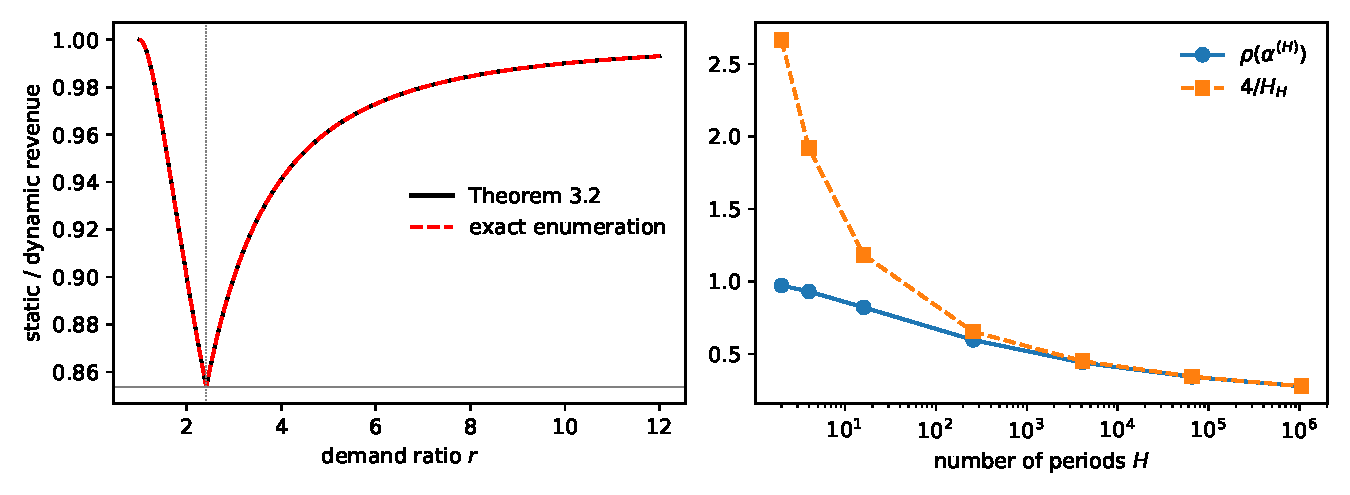
\includegraphics[width=.96\linewidth]{figs/e1.pdf}
\caption{E1. Left: revenue ratio versus demand ratio, Theorem~\ref{thm:known} against exact candidate enumeration. Right: the power-law profile of Theorem~\ref{thm:generalH}(b).}\label{fig:e1}\end{figure}
\begin{table}[t]\centering\small\begin{tabular}{p{0.58\linewidth}rr}
\toprule
Quantity & Prediction & Enumeration \\
\midrule
worst-case ratio $\rho_{\min}$ & 0.853553 & 0.853553 \\
location $r^\ast$ & 2.41421 & 2.41421 \\
max $|\rho_{\rm formula}-\rho_{\rm exact}|$ over grid & 0 & 3.3e-16 \\
violations of $\rho\ge(\sum\alpha)^2/(H\sum\alpha^2)\ge 4mM/(m+M)^2$ in 20{,}000 random profiles & 0 & 0 \\
\bottomrule
\end{tabular}
\vspace{4pt}\begin{tabular}{lrrrr}
\toprule
$H$ & $r=\alpha_{\max}/\alpha_{\min}$ & $\rho(\alpha^{(H)})$ & $4/H_H$ & $\rho\le 4/H_H$ \\
\midrule
2 & 1.4 & 0.9714 & 2.6667 & yes \\
4 & 2.0 & 0.9304 & 1.9200 & yes \\
16 & 4.0 & 0.8210 & 1.1832 & yes \\
256 & 16.0 & 0.5961 & 0.6531 & yes \\
4{,}096 & 64.0 & 0.4395 & 0.4497 & yes \\
65{,}536 & 256.0 & 0.3409 & 0.3428 & yes \\
1{,}048{,}576 & 1024.0 & 0.2766 & 0.2770 & yes \\
\bottomrule
\end{tabular}

\caption{E1. Top: Theorem~\ref{thm:known} against exact enumeration over $6{,}000$ ratios in $[1,50]$ plus a refined grid around $1+\sqrt2$, and the bounds of Theorem~\ref{thm:generalH}(a) on random profiles. Bottom: the power-law profile of Theorem~\ref{thm:generalH}(b) ($\beta=1$); for $H\le4$ the bound $4/H_H$ exceeds one and is vacuous.}\label{tab:e1}\end{table}
The enumeration reproduces the formula of Theorem~\ref{thm:known} to machine precision, with worst case $\EoneMinRho$ at $r=1+\sqrt2$. The bounds of Theorem~\ref{thm:generalH}(a) hold on all $20{,}000$ random profiles, and the power-law profile confirms that the ratio collapses logarithmically in $H$ (Table~\ref{tab:e1}).

\subsection{E2: estimation-error losses and the crossing condition}
Fixed demands $\alpha=(10,8)$, $\beta=1$, i.i.d.\ Gaussian errors, $2\times10^6$ draws per row.
\begin{table}[t]\centering\small\begin{tabular}{rrrrrrrr}
\toprule
$\sigma_\alpha$ & $L^D$ pred. & $L^D$ sim. & $L^S$ pred. & $L^S$ sim. & $L^D\!-\!L^S$ pred. & $L^D\!-\!L^S$ sim. & verified \\
\midrule
0.25 & 0.0312 & 0.0312$\pm$0.0000 & 0.0156 & 0.0156$\pm$0.0000 & 0.0156 & 0.0156$\pm$0.0000 & yes \\
0.50 & 0.1250 & 0.1251$\pm$0.0002 & 0.0625 & 0.0625$\pm$0.0001 & 0.0625 & 0.0625$\pm$0.0001 & yes \\
1.00 & 0.5000 & 0.4999$\pm$0.0007 & 0.2500 & 0.2499$\pm$0.0005 & 0.2500 & 0.2500$\pm$0.0005 & yes \\
1.50 & 1.1250 & 1.1252$\pm$0.0016 & 0.5625 & 0.5629$\pm$0.0011 & 0.5625 & 0.5623$\pm$0.0011 & yes \\
\bottomrule
\end{tabular}

\caption{E2. Revenue arm, Corollary~\ref{cor:rev}. $L^D,L^S$ are losses against their own class oracle under true clipped revenue; ``verified'' applies the reporting standard to all three predictions jointly.}\label{tab:e2iid}\end{table}
\begin{table}[t]\centering\small\begin{tabular}{rrrrrrrr}
\toprule
$\sigma_a$ & $L^D$ pred. & $L^D$ sim. & $L^S$ pred. & $L^S$ sim. & diff pred. & diff sim. & verified \\
\midrule
0.25 & 0.00521 & 0.00520 & 0.00260 & 0.00260 & 0.00260 & 0.00260 & yes \\
0.50 & 0.02083 & 0.02082 & 0.01042 & 0.01042 & 0.01042 & 0.01041 & yes \\
1.00 & 0.08333 & 0.08339 & 0.04167 & 0.04171 & 0.04167 & 0.04168 & yes \\
1.50 & 0.18750 & 0.18762 & 0.09375 & 0.09378 & 0.09375 & 0.09384 & yes \\
\bottomrule
\end{tabular}

\caption{E2/A1. Welfare arm, Corollary~\ref{cor:welf}, $a=(10,8)$, $b=c=1$. The curvature $\lambda=0.375$ from Lemma~\ref{lem:quad}(b) is recovered numerically as $0.3750$ and $G=\kappa(a_1-a_2)^2=1/12$ is matched.}\label{tab:e2w}\end{table}
Tables~\ref{tab:e2iid} and~\ref{tab:e2w} verify the closed forms for revenue and welfare: the dynamic plug-in loses twice the static plug-in's loss, and the difference matches $\sigma^2/(4\beta)$ resp.\ $\kappa(\varepsilon_1-\varepsilon_2)^2$ in expectation.
\begin{figure}[t]\centering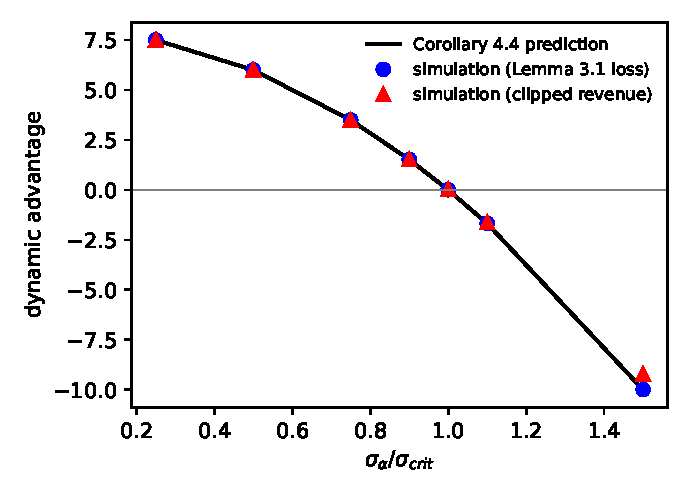
\includegraphics[width=.55\linewidth]{figs/e2.pdf}
\caption{E2. Realized advantage of the dynamic over the static plug-in against error scale, $\alpha=(20,12)$, $\sigma_{\rm crit}=|\alpha_1-\alpha_2|/\sqrt2$ (Corollary~\ref{cor:cross}). The sign flips at $\sigma_{\rm crit}$ under the quadratic loss; under clipped revenue the curve departs from the prediction at and above the crossing.}\label{fig:e2}\end{figure}
\begin{table}[t]\centering\small\begin{tabular}{rrrcrc}
\toprule
$\sigma_\alpha/\sigma_{\rm crit}$ & Corollary 4.4 & sim. (Lemma 3.1 loss) & ok & sim. (clipped revenue) & ok \\
\midrule
0.25 & 7.500 & 7.501$\pm$0.001 & yes & 7.501$\pm$0.001 & yes \\
0.50 & 6.000 & 6.002$\pm$0.004 & yes & 6.002$\pm$0.004 & yes \\
0.75 & 3.500 & 3.499$\pm$0.009 & yes & 3.496$\pm$0.009 & yes \\
0.90 & 1.520 & 1.521$\pm$0.013 & yes & 1.520$\pm$0.012 & yes \\
1.00 & 1.8e-15 & 0.008$\pm$0.016 & yes & 0.025$\pm$0.015 & no \\
1.10 & -1.680 & -1.679$\pm$0.019 & yes & -1.619$\pm$0.018 & no \\
1.50 & -10.000 & -9.995$\pm$0.035 & yes & -9.217$\pm$0.032 & no \\
\bottomrule
\end{tabular}

\caption{E2. Crossing locus. Prediction $G-\sigma_\alpha^2/(4\beta)$ with $G=8$, $\sigma_{\rm crit}=5.657$. The Lemma-1 column is verified in every row. Under clipped revenue the prediction is verified for $\sigma_\alpha<\sigma_{\rm crit}$ and fails at and above it, because errors of size comparable to $\alpha_2=12$ push plug-in tolls into the corner regime (ablation A6).}\label{tab:e2cross}\end{table}
The crossing condition of Corollary~\ref{cor:cross} is confirmed exactly under the quadratic loss; the true-revenue crossing is shifted by corner effects of modest size (Table~\ref{tab:e2cross}), which is the limit of the interior theory.

\subsection{E3: review period}
Random-walk demand, batched cycle-mean policies $m=1,\dots,30$, $1{,}500$ paths of $3{,}000$ days per $m$. Loss is evaluated with the actual revenue function against the oracle static toll.
\begin{figure}[t]\centering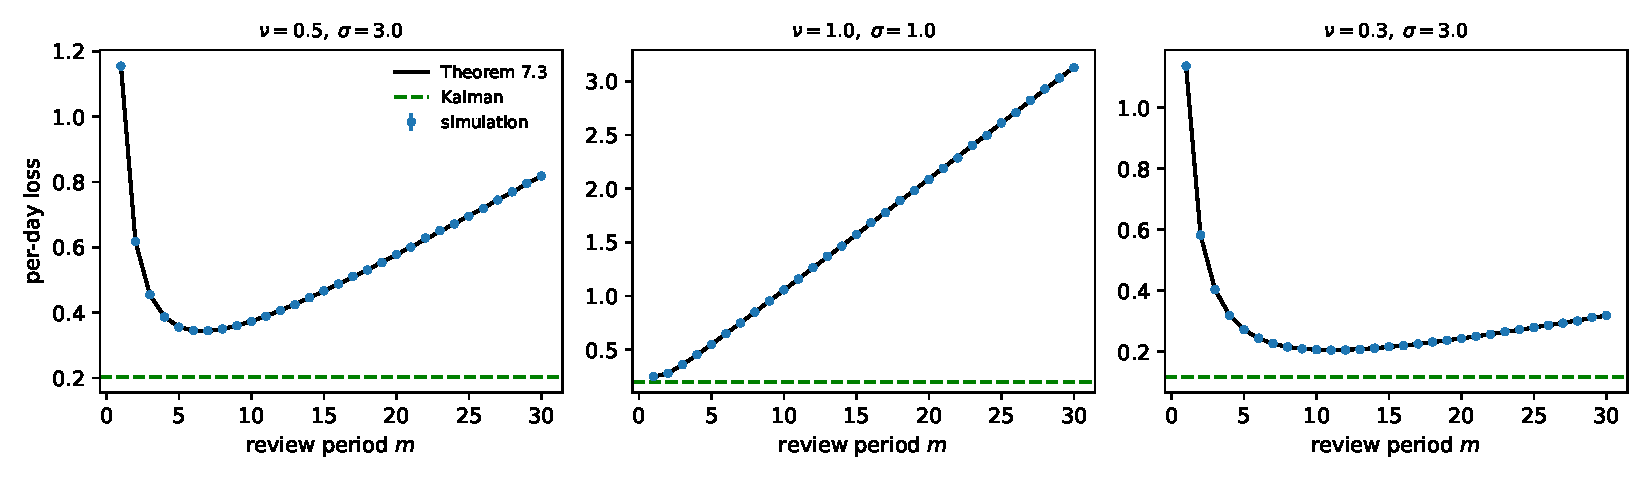
\includegraphics[width=\linewidth]{figs/e3.pdf}
\caption{E3. Per-day loss against review period $m$ for three noise--drift settings: simulation (with $95\%$ CIs) against Theorem~\ref{thm:review}, and the Kalman loss $(p+\nu^2)/(8\beta)$ (dashed).}\label{fig:e3}\end{figure}
\begin{table}[t]\centering\small\begin{tabular}{rrrrrrrrr}
\toprule
$\nu$ & $\sigma$ & $m^\ast$ & int.\ opt.\ pred./sim. & $\bar L(m^\ast)$ & Kalman pred. & Kalman sim. & $m$ verified & max rel.\ err. \\
\midrule
0.5 & 3.0 & 6.59 & 7 / 7 & 0.3431 & 0.2038 & 0.2040$\pm$0.0006 & 29/30 & 0.67\% \\
1.0 & 1.0 & 1.18 & 1 / 1 & 0.2465 & 0.2023 & 0.2023$\pm$0.0003 & 29/30 & 0.58\% \\
0.3 & 3.0 & 10.96 & 11 / 11 & 0.2056 & 0.1183 & 0.1185$\pm$0.0005 & 29/30 & 0.74\% \\
\bottomrule
\end{tabular}

\caption{E3. ``$m$ verified'' counts the cycle lengths $m\in\{1,\dots,30\}$ at which Theorem~\ref{thm:review} is verified under the reporting standard; in each setting the single non-verified $m$ differs from the prediction by less than $0.75\%$ and is a Monte Carlo fluctuation of that size, not a systematic effect (the maximum relative error over all $m$ is in the last column).}\label{tab:e3}\end{table}
\begin{table}[t]\centering\small\begin{tabular}{rrrcc}
\toprule
$\sigma^2/\nu^2$ & $m^\ast$ (relaxed) & best integer $m$ & predicted $m{=}1$ & consistent \\
\midrule
0.50 & 0.894 & 1 & yes & yes \\
1.00 & 1.183 & 1 & yes & yes \\
1.40 & 1.371 & 1 & yes & yes \\
1.50 & 1.414 & 1 & yes & yes \\
1.60 & 1.456 & 2 & no & yes \\
2.00 & 1.612 & 2 & no & yes \\
4.00 & 2.236 & 2 & no & yes \\
9.00 & 3.317 & 3 & no & yes \\
\bottomrule
\end{tabular}

\caption{E3. Corollary~\ref{cor:daily}: daily batching is optimal over integers iff $\sigma^2/\nu^2\le3/2$ (exact evaluation of Theorem~\ref{thm:review}).}\label{tab:cor4}\end{table}
Theorem~\ref{thm:review} is verified at $29$ of $30$ cycle lengths in each of the three settings, the integer optimum is predicted exactly, and Corollary~\ref{cor:daily} is consistent with exact evaluation (Table~\ref{tab:cor4}). With revision cost $C=0.2$ at $\nu=0.5,\sigma=3,\beta=1$ the cost-adjusted optimum is $m^*=7.15$ and the best integer period is $7$ (Corollary~\ref{cor:cost}).

\paragraph{Filtering versus batching (Theorem~\ref{thm:kalman}).}
\begin{table}[t]\centering\small\begin{tabular}{rrrrc}
\toprule
$m$ & cycle-mean (Thm.~\ref{thm:review}) & Kalman-scheduled pred. & Kalman-scheduled sim. & dominates \\
\midrule
1 & 1.1562 & 0.2038 & 0.2040$\pm$0.0006 & yes \\
2 & 0.6172 & 0.2194 & 0.2197$\pm$0.0007 & yes \\
4 & 0.3867 & 0.2506 & 0.2510$\pm$0.0008 & yes \\
8 & 0.3496 & 0.3131 & 0.3135$\pm$0.0011 & yes \\
\bottomrule
\end{tabular}

\caption{E3. $\nu=0.5$, $\sigma=3$, $\beta=1$ (no revision cost). Kalman-scheduled loss $[p+(m+1)\nu^2/2]/(8\beta)$ with $p=1.380$ against the cycle-mean loss of Theorem~\ref{thm:review}.}\label{tab:ksched}\end{table}
\begin{table}[t]\centering\small\begin{tabular}{rrr}
\toprule
gain $g$ & closed form & simulation \\
\midrule
0.02 & 0.8005 & 0.7941$\pm$0.0080 \\
0.05 & 0.3494 & 0.3486$\pm$0.0022 \\
0.10 & 0.2237 & 0.2237$\pm$0.0010 \\
0.20 & 0.2118 & 0.2121$\pm$0.0006 \\
0.30 & 0.2598 & 0.2598$\pm$0.0006 \\
0.50 & 0.4167 & 0.4165$\pm$0.0008 \\
0.80 & 0.7826 & 0.7826$\pm$0.0011 \\
1.00 & 1.1562 & 1.1566$\pm$0.0016 \\
\bottomrule
\end{tabular}

\caption{E3. EWMA with gain $g$ (Proposition~\ref{prop:ewma}), $\nu=0.5$, $\sigma=3$; the minimum is at $g^*=0.153$ with loss $0.2038$.}\label{tab:ewma}\end{table}
Table~\ref{tab:ksched} confirms Theorem~\ref{thm:kalman}: the Kalman-scheduled loss matches its formula and is below the cycle-mean loss at every $m$. At $\nu=0.5$, $\sigma=3$ the batched optimum is $0.343$ and the Kalman filter achieves $0.204$, a $41\%$ reduction; even in the high-drift setting $\nu=\sigma=1$ where daily batching is optimal in its class ($0.2465$) the filter achieves $0.2023$. Table~\ref{tab:ewma} confirms the closed form for the EWMA family.

\subsection{E4: recovery from a demand shift and CUSUM (A4)}
\begin{table}[t]\centering\small\begin{tabular}{rrrr}
\toprule
$m$ & $(3m-1)/2$ & enumerated mean & range \\
\midrule
1 & 1.0 & 1.0 & 1--1 \\
2 & 2.5 & 2.5 & 2--3 \\
3 & 4.0 & 4.0 & 3--5 \\
5 & 7.0 & 7.0 & 5--9 \\
8 & 11.5 & 11.5 & 8--15 \\
12 & 17.5 & 17.5 & 12--23 \\
20 & 29.5 & 29.5 & 20--39 \\
30 & 44.5 & 44.5 & 30--59 \\
\bottomrule
\end{tabular}

\caption{E4. Days until the toll is based solely on post-jump data, enumerated over \emph{every} jump offset in a cycle, noise-free (Proposition~\ref{prop:recovery}).}\label{tab:lag}\end{table}
The enumeration in Table~\ref{tab:lag} matches $(3m-1)/2$ exactly. The estimate-once policy ($25$ initial days, $\sigma=2$, $\Delta=3$) has post-jump per-day loss \EfourOnceSim{} against the prediction \EfourOncePred.
\begin{table}[t]\centering\small\begin{tabular}{rrrrrrr}
\toprule
$\Delta/\sigma$ & $m$ & scheduled & CUSUM+scheduled & detect rate & delay (days) & pre-jump false alarm \\
\midrule
2.0 & 10 & 0.0281 & 0.0283 & 0.981 & 5.91 & 0.018 \\
2.0 & 30 & 0.0477 & 0.0250 & 1.000 & 4.76 & 0.046 \\
4.0 & 10 & 0.0749 & 0.0627 & 1.000 & 1.67 & 0.021 \\
4.0 & 30 & 0.1774 & 0.0624 & 1.000 & 1.67 & 0.046 \\
\bottomrule
\end{tabular}

\caption{A4. Change-point detection. Per-day loss over $300$ post-jump days ($\sigma=1$, no drift), $6{,}000$ paths per row, CUSUM with allowance $k=0.5\sigma$ and threshold $h=8\sigma$; after an alarm the planner waits $5$ days and re-estimates from them. Detection delay is measured from the jump, among detected jumps.}\label{tab:cusum}\end{table}
Table~\ref{tab:cusum} shows that adding a CUSUM detector to a long review period ($m=30$) reduces post-jump loss to about $1/1.9$ (approximately $0.52$ times the scheduled loss) for $\Delta=2\sigma$, and to about $1/2.8$ (approximately $0.35$ times the scheduled loss) for $\Delta=4\sigma$, at no cost in the stationary regime (no-jump loss $\EfourNJc$ against $\EfourNJs$). For $m=10$ and a small jump the detector brings no gain. The price is a false-alarm rate of about $\EfourFA$ over $300$ no-jump days for $m=30$; the threshold $h$ trades it off against delay. Detection therefore substitutes for scheduling when the jump is large relative to noise.

\subsection{E5: identifiability}
Example~\ref{ex:ident} is simulated directly. Under an \emph{adaptive} interior toll rule (tolls feed back on past observations, clipped to keep both periods active in both profiles) the observation process is indistinguishable: over $30$ days and $4\times10^4$ paths, the smallest two-sample Kolmogorov--Smirnov $p$-value across days is $\EfiveIntKS$ (consistent with the minimum of $30$ draws under the null) and the pooled mean gap is $0.0015$ for noise standard deviation $1$. At the corner probe $(5.5,5.5)$ the profiles separate; the accuracy of the optimal test against probe days matches $\Phi(\Delta\mu\sqrt n/2\sigma)$ (Table~\ref{tab:corner}) while each probe day forgoes $4.5$ or $1.75$ revenue (Remark~\ref{rem:corner-probe}). With per-period sensors (O2) the split is recovered at standard error $\EfiveSE$ after $25$ days against the predicted $0.2$.
\begin{table}[t]\centering\small\begin{tabular}{rrr}
\toprule
probe days $n$ & predicted accuracy $\Phi(\Delta\mu\sqrt n/2\sigma)$ & simulated accuracy \\
\midrule
1 & 0.5987 & 0.6001 \\
4 & 0.6915 & 0.6914 \\
16 & 0.8413 & 0.8416 \\
64 & 0.9772 & 0.9777 \\
144 & 0.9987 & 0.9987 \\
\bottomrule
\end{tabular}

\caption{E5. Accuracy of the likelihood-ratio test between $\alpha=(10,6)$ and $\alpha'=(11,5)$ from $n$ days of corner probes, $\sigma=1$ ($10^5$ replications).}\label{tab:corner}\end{table}

\subsection{Ablations}
\paragraph{A2: error structure.} Table~\ref{tab:a2} varies correlation, tail weight and bias. Correlation and bias predictions of Remark~\ref{rem:corr} are verified in all nine rows. The Student-$t_3$ arm is the exception: the simulated difference $0.2388\pm0.0094$ lies $4.5\%$ below the prediction $0.25$. This is not a failure of Theorem~\ref{thm:est}, whose expectation requires only finite variance; it reflects clipping, since heavy-tailed errors of this scale occasionally exceed $\alpha_2=8$ and push tolls into the corner regime. We report it as an unverified arm.
\begin{table}[t]\centering\small\begin{tabular}{lrrc}
\toprule
Error structure & Prediction of $E[L^D-L^S]$ & Simulation & verified \\
\midrule
correlation $\rho=-1$ & 0.5000 & 0.5001$\pm$0.0014 & yes \\
correlation $\rho=-0.5$ & 0.3750 & 0.3747$\pm$0.0010 & yes \\
correlation $\rho=0$ & 0.2500 & 0.2500$\pm$0.0007 & yes \\
correlation $\rho=0.5$ & 0.1250 & 0.1249$\pm$0.0003 & yes \\
correlation $\rho=1$ & 0.0000 & 0.0000$\pm$0.0000 & yes \\
Student-$t_3$ errors & 0.2500 & 0.2388$\pm$0.0094 & no \\
bias $(+0.5,+0.5)$ & 0.2500 & 0.2498$\pm$0.0007 & yes \\
bias $(+1.0,+1.0)$ & 0.2500 & 0.2497$\pm$0.0007 & yes \\
bias $(+0.5,-0.5)$ & 0.3750 & 0.3742$\pm$0.0010 & yes \\
bias $(+1.0,-1.0)$ & 0.7500 & 0.7496$\pm$0.0015 & yes \\
\bottomrule
\end{tabular}

\caption{A2. Ablation over error structure, $\alpha=(10,8)$, $\sigma_\alpha=1$, $10^6$ draws.}\label{tab:a2}\end{table}
\paragraph{A6: corners.} Table~\ref{tab:a6} shows what happens when errors become large relative to demand ($\alpha=(6,3)$). The interior theory is accurate to $0.4\%$ at $\sigma_\alpha=0.5$ and drifts by $2.7\%$ at $\sigma_\alpha=1$; the sign of the deviation changes between $\sigma_\alpha=2$ and $3$, and at $\sigma_\alpha=4$ the true difference is $13\%$ below the quadratic prediction. The qualitative ordering $L^D\ge L^S$ is preserved throughout in expectation.
\begin{table}[t]\centering\small\begin{tabular}{rrrr}
\toprule
$\sigma_\alpha$ & Lemma-1 prediction & clipped revenue & rel.\ deviation \\
\midrule
0.5 & 0.0625 & 0.0627$\pm$0.0002 & +0.4\% \\
1.0 & 0.2500 & 0.2567$\pm$0.0007 & +2.7\% \\
2.0 & 1.0000 & 1.0754$\pm$0.0027 & +7.5\% \\
3.0 & 2.2500 & 2.2195$\pm$0.0054 & -1.4\% \\
4.0 & 4.0000 & 3.4616$\pm$0.0086 & -13.5\% \\
\bottomrule
\end{tabular}

\caption{A6. $E[L^D-L^S]$ under clipped true revenue against the Lemma-1 prediction $\sigma_\alpha^2/(4\beta)$, $\alpha=(6,3)$.}\label{tab:a6}\end{table}
\paragraph{A7: number of periods.} Table~\ref{tab:a7} varies $H$ with demand profile $\alpha_i=\mathrm{linspace}(14,10,H)$ and i.i.d.\ errors. The dynamic plug-in loses $H\sigma^2/(4\beta)$ and the static one $\sigma^2/(4\beta)$, so the static advantage grows with $H$ and the crossing threshold is $(H-1)\sigma^2/(4\beta)$ (Theorem~\ref{thm:shrink}(b)). Three of four rows are verified; at $H=16$ the static loss is $0.2486$ against $0.25$ ($0.56\%$), just outside the $0.5\%$ tolerance, and is reported as unverified.
\begin{table}[t]\centering\small\begin{tabular}{rrrrrrrr}
\toprule
$H$ & $E L^D$ pred. & sim. & $E L^S$ pred. & sim. & $G$ & threshold $(H\!-\!1)\sigma^2/4\beta$ & dynamic wins \\
\midrule
2 & 0.500 & 0.500 & 0.250 & 0.250 & 2.000 & 0.250 & yes \\
4 & 1.000 & 0.999 & 0.250 & 0.250 & 2.222 & 0.750 & yes \\
8 & 2.000 & 1.997 & 0.250 & 0.251 & 3.429 & 1.750 & yes \\
16 & 4.000 & 3.997 & 0.250 & 0.249 & 6.044 & 3.750 & yes \\
\bottomrule
\end{tabular}

\caption{A7. Number of periods, $\sigma=1$, $\beta=1$. ``dynamic wins'' is $G$ against the threshold.}\label{tab:a7}\end{table}

\paragraph{A3: demand dynamics.} Table~\ref{tab:a3} compares dynamics for $\nu=0.5$, $\sigma=3$. Mean reversion strongly lengthens the best review period: for $\phi=0.8$ the best period is the largest in our grid ($60$), because with a stationary mean longer averaging only helps. For deterministic drift the cube-root law of Proposition~\ref{prop:drift} predicts the integer optimum exactly. With weekly seasonality, calendar-aligned weekday means (four weeks) reach the noise floor $\sigma^2/(4\cdot8\beta)=0.125$, far below any cycle-mean policy: the best cycle policy ($m=14$) loses $0.598$.
\begin{table}[t]\centering\small
\begin{minipage}[t]{.48\linewidth}\centering\begin{tabular}{rrrr}
\toprule
$\phi$ & best $m$ & loss at best $m$ & loss at $m{=}1$ \\
\midrule
1.0 & 6 & 0.3435 & 1.1566 \\
0.99 & 7 & 0.3375 & 1.1572 \\
0.95 & 8 & 0.3115 & 1.1583 \\
0.8 & $\ge 60$ & 0.1168 & 1.1588 \\
\bottomrule
\end{tabular}
\end{minipage}\hfill
\begin{minipage}[t]{.48\linewidth}\centering\begin{tabular}{lr}
\toprule
Policy & per-day loss \\
\midrule
cycle mean, $m=1$ & 0.9230 \\
cycle mean, $m=2$ & 1.4699 \\
cycle mean, $m=3$ & 1.6121 \\
cycle mean, $m=7$ & 0.6338 \\
cycle mean, $m=14$ & 0.5980 \\
weekday mean, $w=2$ weeks & 0.2498 \\
weekday mean, $w=4$ weeks & 0.1247 \\
weekday mean, $w=8$ weeks & 0.0623 \\
\bottomrule
\end{tabular}
\end{minipage}\vspace{6pt}
\begin{tabular}{rrrrr}
\toprule
$\delta$ & $m^\ast=(6\sigma^2/13\delta^2)^{1/3}$ & best int.\ pred. & best int.\ sim. & max rel.\ err. \\
\midrule
0.05 & 9.039 & 9 & 9 & 1.02\% \\
0.10 & 5.694 & 6 & 6 & 0.41\% \\
0.20 & 3.587 & 4 & 4 & 0.57\% \\
\bottomrule
\end{tabular}

\caption{A3. Left: AR(1) demand. Right: weekly seasonality ($A=3$, $\sigma=2$). Bottom: deterministic drift ($\sigma=2$), Proposition~\ref{prop:drift}.}\label{tab:a3}\end{table}

\paragraph{A5/A8: unknown slope and heteroskedastic noise.} Table~\ref{tab:a5} verifies the exact variances of Proposition~\ref{prop:slope} for $\hat\beta$ and $\hat S$ and shows that the first-order variance of $\hat\tau$ is accurate to about $2\%$ at $\delta=2$ but underestimates by up to $26\%$ at $\delta=0.5$ (second-order terms), the $1/\delta^2$ cost the proposition describes. With noise proportional to flow ($\kappa=0.1$) Table~\ref{tab:a8} shows that $\Var(\hat\tau)$ still falls steeply with the centre $\bar\tau$, so the conclusion that higher-centered probes are cheaper does \emph{not} flip in the range tested.
\begin{table}[t]\centering\small\begin{tabular}{rrrrrrrr}
\toprule
$\bar\tau$ & $\delta$ & Var$\hat\beta$ pred. & sim. & Var$\hat S$ pred. & sim. & Var$\hat\tau$ 1st-order & sim. \\
\midrule
2.0 & 0.5 & 0.02500 & 0.02500 & 0.4250 & 0.4249 & 0.2266 & 0.2861 \\
2.0 & 1.0 & 0.00625 & 0.00625 & 0.1250 & 0.1248 & 0.0578 & 0.0608 \\
2.0 & 2.0 & 0.00156 & 0.00156 & 0.0500 & 0.0498 & 0.0156 & 0.0158 \\
3.0 & 0.5 & 0.02500 & 0.02505 & 0.9250 & 0.9265 & 0.1578 & 0.1989 \\
3.0 & 1.0 & 0.00625 & 0.00624 & 0.2500 & 0.2501 & 0.0406 & 0.0426 \\
3.0 & 2.0 & 0.00156 & 0.00156 & 0.0813 & 0.0811 & 0.0113 & 0.0114 \\
4.0 & 0.5 & 0.02500 & 0.02493 & 1.6250 & 1.6211 & 0.1016 & 0.1274 \\
4.0 & 1.0 & 0.00625 & 0.00626 & 0.4250 & 0.4260 & 0.0266 & 0.0279 \\
4.0 & 2.0 & 0.00156 & 0.00156 & 0.1250 & 0.1247 & 0.0078 & 0.0079 \\
\bottomrule
\end{tabular}

\caption{A5. Two-level probing, $S=16$, $\sigma=1$, $n=20$, $4\times10^5$ replications. The first-order formula for $\Var(\hat\tau)$ is a delta-method approximation.}\label{tab:a5}\end{table}
\begin{table}[t]\centering\small\begin{tabular}{rrrr}
\toprule
$\bar\tau$ & const.-noise formula & delta method (prop.\ noise) & simulation \\
\midrule
1.0 & 0.0781 & 0.1440 & 0.1613 \\
2.0 & 0.0578 & 0.0766 & 0.0828 \\
3.0 & 0.0406 & 0.0360 & 0.0380 \\
4.0 & 0.0266 & 0.0141 & 0.0145 \\
5.0 & 0.0156 & 0.0040 & 0.0041 \\
\bottomrule
\end{tabular}

\caption{A8. Noise standard deviation $\kappa\times$flow ($\kappa=0.1$), $\delta=1$, $n=20$. The delta method with heteroskedastic covariance tracks simulation; the constant-noise formula does not.}\label{tab:a8}\end{table}

\subsection{E7: shrinkage between static and dynamic}
\begin{figure}[t]\centering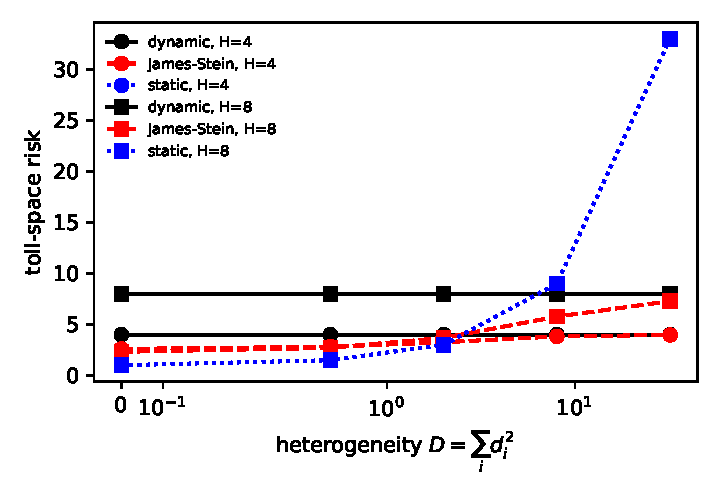
\includegraphics[width=.6\linewidth]{figs/e7.pdf}
\caption{E7. Toll-space risk against heterogeneity $D$ for the static, dynamic and James--Stein estimators, $H=4,8$, $s=1$.}\label{fig:e7}\end{figure}
\begin{table}[t]\centering\small\begin{tabular}{rrrrrrrr}
\toprule
$H$ & $D$ & static & dynamic & oracle $w^\ast$ (pred.) & oracle $w^\ast$ (sim.) & plug-in PP & James--Stein \\
\midrule
2 & 0.0 & 1.001 & 2.001 & 1.000 & 1.001 & 1.334 & -- \\
2 & 2.0 & 2.997 & 1.999 & 1.667 & 1.666 & 2.180 & -- \\
2 & 8.0 & 9.003 & 2.002 & 1.889 & 1.890 & 2.445 & -- \\
2 & 32.0 & 33.002 & 2.003 & 1.970 & 1.972 & 2.107 & -- \\
4 & 0.0 & 0.997 & 3.994 & 1.000 & 0.997 & 1.495 & 2.597 \\
4 & 2.0 & 2.996 & 3.990 & 2.200 & 2.195 & 2.785 & 3.255 \\
4 & 8.0 & 9.001 & 3.998 & 3.182 & 3.180 & 4.079 & 3.827 \\
4 & 32.0 & 33.002 & 3.998 & 3.743 & 3.742 & 4.097 & 3.966 \\
8 & 0.0 & 1.002 & 7.995 & 1.000 & 1.002 & 1.617 & 2.318 \\
8 & 2.0 & 3.002 & 7.993 & 2.556 & 2.557 & 3.205 & 3.683 \\
8 & 8.0 & 9.000 & 8.002 & 4.733 & 4.732 & 5.791 & 5.766 \\
8 & 32.0 & 32.998 & 7.985 & 6.744 & 6.739 & 7.397 & 7.281 \\
16 & 0.0 & 1.003 & 16.018 & 1.000 & 1.003 & 1.717 & 2.214 \\
16 & 2.0 & 3.000 & 15.988 & 2.765 & 2.765 & 3.480 & 3.889 \\
16 & 8.0 & 8.998 & 15.993 & 6.217 & 6.213 & 7.294 & 7.407 \\
16 & 32.0 & 32.995 & 16.001 & 11.213 & 11.211 & 12.206 & 12.116 \\
\bottomrule
\end{tabular}

\caption{E7. Toll-space risk $\E\|\hat\tau(w)-\tau^*\|^2$, $s=1$, $4\times10^5$ draws. ``plug-in PP'' uses $w=(1-(H-1)s^2/\|\hat\tau-\bar{\hat\tau}\|^2)_+$; James--Stein uses $(H-3)$ and is defined for $H\ge4$. The closed forms of Theorem~\ref{thm:shrink}(a),(b) are matched to Monte Carlo error.}\label{tab:e7}\end{table}
The oracle-weight risk matches Theorem~\ref{thm:shrink}(b) in every cell, and the James--Stein weight beats the dynamic plug-in in every cell with $H\ge4$ (Table~\ref{tab:e7}), as the theory predicts. For $H=2$ the plug-in positive-part rule beats the dynamic plug-in when heterogeneity is small ($D\le0.5$) but \emph{not} when it is moderate ($D\in\{2,8\}$), where it is up to $22\%$ worse: dominance needs $H\ge4$, and we do not claim it for $H=2$.

\subsection{E8: coupled periods}
Theorem~\ref{thm:coupled} is tested directly with $H=6$ periods, $B=\beta I+\kappa\mathcal L$ with $\kappa\in\{0,0.5,2,8\}$, $\beta=1$, correlated Gaussian errors with random covariance, $10^5$ draws per row; $L^D$ and $L^S$ are computed from the revenue function directly, not from the closed forms.
\begin{table}[t]\centering\small\begin{tabular}{rrrrrrrrr}
\toprule
$\kappa$ & cond$(B)$ & max err $L^D$ & max err $L^S$ & min $L^D\!-\!L^S$ & frac.\ $<0$ & $G$ & mean gap & formula \\
\midrule
0.0 & 1.0 & 1.5e-13 & 1.4e-13 & 0.00075 & 0.0 & 3.353 & 0.4992 & 0.4992 \\
0.5 & 2.9 & 3.7e-13 & 2.6e-13 & 0.00081 & 0.0 & 5.586 & 0.4007 & 0.4007 \\
2.0 & 8.5 & 3.0e-13 & 2.7e-13 & 0.00028 & 0.0 & 2.402 & 0.2469 & 0.2469 \\
8.0 & 30.9 & 1.1e-12 & 8.5e-13 & 0.00008 & 0.0 & 0.789 & 0.0302 & 0.0302 \\
\bottomrule
\end{tabular}

\caption{E8. Theorem~\ref{thm:coupled}: the maximal deviation of directly computed losses from the closed forms is at the level of floating-point error ($<2\times10^{-12}$); $L^D-L^S$ is never negative; on the direction $\varepsilon\propto B\one$ the gap vanishes (to $10^{-13}$).}\label{tab:e8}\end{table}
Table~\ref{tab:e8} confirms Theorem~\ref{thm:coupled} as an identity and not merely in expectation, for substitution strengths covering a condition number from $1$ to $31$.

\subsection{E9: certainty equivalence at the corner}
\begin{table}[t]\centering\small\begin{tabular}{rrrrrr}
\toprule
$s/\mu$ & plug-in toll & Bayes toll & exp.\ rev.\ plug-in & exp.\ rev.\ Bayes & gain \\
\midrule
0.05 & 5.000 & 4.998 & 25.000 & 25.000 & -0.000\% \\
0.20 & 5.000 & 5.018 & 25.020 & 25.020 & 0.001\% \\
0.40 & 5.000 & 5.483 & 26.012 & 26.187 & 0.672\% \\
0.60 & 5.000 & 6.368 & 28.399 & 29.518 & 3.938\% \\
\bottomrule
\end{tabular}

\caption{E9. Bayes-optimal versus plug-in single-period toll under posterior $\alpha\sim N(\mu,s^2)$, $\mu=10$, $\beta=1$, true clipped revenue. Rows with $s/\mu>0.6$ are omitted because the Gaussian posterior then places non-negligible mass on negative demand.}\label{tab:e9}\end{table}
Table~\ref{tab:e9} illustrates Remark~\ref{rem:corners}: the Bayes toll equals the plug-in toll in the interior regime and exceeds it as posterior uncertainty grows, with gains of order $4\%$ of revenue at $s/\mu=0.6$.

\subsection{Scorecard}
Of the closed forms tested, Theorems~\ref{thm:known}, \ref{thm:generalH}, \ref{thm:est}--\ref{thm:shrink}(a,b), \ref{thm:review}, \ref{thm:kalman} and Propositions~\ref{prop:ident-static}--\ref{prop:recovery} are verified under the reporting standard in the interior regime. The tested arms that are \emph{not} verified are: the true-revenue crossing at and above $\sigma_{\rm crit}$ (three rows), Student-$t_3$ errors, $H=16$ in A7, and a single cycle length per setting in E3 (within $0.75\%$); all trace to clipping, heavy tails or Monte Carlo fluctuation of sub-percent size. The first-order $\Var(\hat\tau)$ of Proposition~\ref{prop:slope} is an approximation by construction and is reported as such. The Bayes-at-corners claim is exploratory (a numerical illustration, not a theorem).

\end{expsec}

\section{Related work}\label{sec:related}
\paragraph{Simple versus optimal congestion pricing.} The starting point is Jalota, Di and Elmachtoub~\cite{jde2026}, whose known-demand guarantees (static tolls achieve a constant fraction of dynamic optimal revenue and at most twice the minimum system cost in bottleneck and MFD models) our Theorems~\ref{thm:known} and~\ref{thm:generalH} parallel in a reduced model; we add the demand-learning dimension they do not treat. Vickrey's bottleneck model~\cite{vickrey1969} is the canonical departure-time framework our Conjecture~\ref{conj:bottle} targets, and Pigou's marginal-cost tolls~\cite{pigou1920} are the welfare benchmark of Lemma~\ref{lem:quad}(b).
\paragraph{Learning tolls and prices.} Jalota, Gopalakrishnan, Azizan, Johari and Pavone~\cite{jalota2023routing} learn tolls from observed aggregate flows with $O(\sqrt T)$ regret against a complete-information oracle, and Chiu and Sastry~\cite{chiu2024} learn latency and choice parameters while tolling, also with $\tilde O(\sqrt T)$ regret. These works learn toward the optimal toll; none compares simple and flexible policy classes under estimation error (our Theorems~\ref{thm:est}--\ref{thm:shrink}) or characterises update frequency (our Theorems~\ref{thm:review}--\ref{thm:kalman}). Jalota, Sun and Azizan~\cite{jalota2023eq} study learning prices with unknown supplier costs in markets without congestion feedback.
\paragraph{Dynamic pricing with demand learning.} The revenue-management literature (survey: den Boer~\cite{denboer2015}) studies pricing while learning demand. Besbes and Zeevi~\cite{besbes2015} show that linear models suffice for near-optimal pricing, which supports our linear-demand assumption. Keskin and Zeevi~\cite{keskin2017} design near-optimal policies for a product whose demand changes under a variation budget; our random walk is a smoothly changing special case and Theorem~\ref{thm:review} is a scheduled-estimation counterpart with the toll-specific coupling that observations are shaped by the price itself. Static-versus-dynamic comparisons also appear in Fisher markets~\cite{jalotaye2024}, and static-pricing guarantees for reusable resources and queues~\cite{besbes2024static,bergquist2023} bound the static/dynamic gap under \emph{known} stochastic demand, a different source of gap from the estimation error studied here. Time-varying tolls with elastic demand in the bottleneck model are analysed by Verhoef~\cite{verhoef1997}; we do not claim our identifiability statements (Section~\ref{sec:ident}), which concern demand levels in a reduced model, extend or contradict that analysis.
\paragraph{Statistical tools.} Theorem~\ref{thm:shrink} uses the James--Stein phenomenon~\cite{jamesstein1961,lindley1962} and its empirical-Bayes interpretation~\cite{efronmorris1973}; Theorem~\ref{thm:kalman} uses the Kalman filter~\cite{kalman1960} and the classical fact that exponential smoothing is optimal for a random walk observed with noise~\cite{muth1960}; the change-point arm uses Page's CUSUM~\cite{page1954}. We have not found the specific static-versus-dynamic toll comparison under estimation error, the crossing condition of Corollary~\ref{cor:cross}, the review-period formulas, or the Kalman-with-revision-costs comparison in the literature.

\section{Scope, limitations and open problems}\label{sec:open}
\begin{enumerate}[label=\textbf{L\arabic*.}]
\item \textbf{Reduced form.} The base model replaces departure-time choice with a static within-period externality. Section~\ref{sec:coupled} adds linear cross-period substitution; nothing here is a statement about the bottleneck model until Conjecture~\ref{conj:bottle} is proved.
\item \textbf{Interior regime.} Theorems~\ref{thm:est}, \ref{thm:coupled}, \ref{thm:bayes} assume non-binding non-negativity. Large errors drive plug-in tolls to corners (A6, E9); a corner-aware Bayes theory is open.
\item \textbf{Known slope.} $\beta$ is known except in Proposition~\ref{prop:slope}. Optimal probe design and a regret theorem for the dynamic objective are open.
\item \textbf{First models.} Random walk demand, i.i.d.\ noise and Gaussian-prior shrinkage are first models; A3 shows how conclusions move under mean reversion, drift and seasonality, but no closed form is given for mean reversion.
\item \textbf{Objectives.} Revenue and welfare share the same algebra; equity, transit-agency revenue allocation and political constraints are not modeled.
\end{enumerate}
\begin{conjecture}[Bottleneck extension]\label{conj:bottle}
In Vickrey's bottleneck model with a public-transit outside option, the oracle static and dynamic revenue-optimal tolls are locally well approximated as linear in the demand scale, and the robustness ordering of Theorem~\ref{thm:est} persists: demand-estimation error degrades the optimal time-varying toll at least as much as the optimal static toll, with the crossing governed by the error in the estimated toll differential. Supporting structure: the static toll also depends on demand through a one-dimensional aggregate, while the dynamic toll depends on the demand profile. Theorem~\ref{thm:coupled} proves the analogue under linear cross-period substitution. Unproved in the bottleneck model.
\end{conjecture}
\begin{conjecture}[MFD extension]\label{conj:mfd}
The analogous ordering holds in the city-scale MFD model of~\cite{jde2026} under learned demand, with weaker constants, mirroring their known-demand finding that MFD guarantees are weaker than bottleneck guarantees. Unproved and untested.
\end{conjecture}

\section{Practical summary}\label{sec:practice}
\begin{itemize}
\item \emph{Only aggregate counts are available?} Use a static toll; the dynamic-optimal toll is not identifiable from interior aggregate flows (Proposition~\ref{prop:ident-split}).
\item \emph{Period-resolved sensing is available?} Estimate the toll differential with shrinkage (Theorem~\ref{thm:shrink}): the weight $w^*=D/(D+(H-1)s^2)$ interpolates, and the naive dynamic plug-in is dominated for $H\ge4$ (James--Stein).
\item \emph{Review frequency?} Random-walk drift gives $m^*\approx(\sigma/\nu)\sqrt{6/5}$; deterministic drift gives $m^*=(6\sigma^2/(13\delta^2))^{1/3}$. Revision costs add $48\beta C$ under the square root.
\item \emph{Can the planner filter?} A Kalman/EWMA estimate attains $m_K^*=4\sqrt{\beta C}/\nu$, with review frequency set by revision cost (Theorem~\ref{thm:kalman}).
\item \emph{Long review period but occasional shocks?} Add a change-point detector (A4).
\end{itemize}

\section*{Acknowledgments}
This paper builds on the framework of Jalota, Di and Elmachtoub~\cite{jde2026}. The author is not affiliated with those authors, and any errors are the author's alone. The views expressed are the author's and do not necessarily reflect those of Microsoft.
% ACK-PLACEHOLDER: add names of colleagues who have agreed to be acknowledged.

\bibliographystyle{plain}
\begin{thebibliography}{99}
\bibitem{jde2026} D.~Jalota, S.~Di, A.~N.~Elmachtoub. \emph{Simple vs.\ Optimal Congestion Pricing}. arXiv:2602.21495, 2026.
\bibitem{vickrey1969} W.~S.~Vickrey. Congestion theory and transport investment. \emph{American Economic Review} 59(2):251--260, 1969.
\bibitem{pigou1920} A.~C.~Pigou. \emph{The Economics of Welfare}. Macmillan, 1920.
\bibitem{jalota2023routing} D.~Jalota, K.~Gopalakrishnan, N.~Azizan, R.~Johari, M.~Pavone. Online learning for traffic routing under unknown preferences. \emph{AISTATS}, PMLR vol.~206, pp.~3210--3229, 2023.
\bibitem{chiu2024} C.-Y.~Chiu, S.~Sastry. Parameter estimation in optimal tolling for traffic networks under the Markovian traffic equilibrium. \emph{American Control Conference}, 2024; arXiv:2409.19765.
\bibitem{jalota2023eq} D.~Jalota, H.~Sun, N.~Azizan. Online learning for equilibrium pricing in markets under incomplete information. arXiv:2303.11522, 2023.
\bibitem{jalotaye2024} D.~Jalota, Y.~Ye. Stochastic online Fisher markets: static pricing limits and adaptive enhancements. \emph{Operations Research} 73(2):798--818, 2025; arXiv:2205.00825.
\bibitem{denboer2015} A.~V.~den Boer. Dynamic pricing and learning: historical origins, current research, and new directions. \emph{Surveys in Operations Research and Management Science} 20(1):1--18, 2015.
\bibitem{besbes2015} O.~Besbes, A.~Zeevi. On the (surprising) sufficiency of linear models for dynamic pricing with demand learning. \emph{Management Science} 61(4):723--739, 2015.
\bibitem{keskin2017} N.~B.~Keskin, A.~Zeevi. Chasing demand: learning and earning in a changing environment. \emph{Mathematics of Operations Research} 42(2):277--307, 2017.
\bibitem{jamesstein1961} W.~James, C.~Stein. Estimation with quadratic loss. In \emph{Proc.\ Fourth Berkeley Symposium on Mathematical Statistics and Probability}, vol.~1, pp.~361--379, 1961.
\bibitem{lindley1962} D.~V.~Lindley. Discussion on Professor Stein's paper. \emph{J.\ Roy.\ Statist.\ Soc.\ Ser.~B} 24(2):285--287, 1962.
\bibitem{efronmorris1973} B.~Efron, C.~Morris. Stein's estimation rule and its competitors---an empirical Bayes approach. \emph{J.\ Amer.\ Statist.\ Assoc.} 68(341):117--130, 1973.
\bibitem{besbes2024static} O.~Besbes, A.~N.~Elmachtoub, Y.~Sun. Static pricing: universal guarantees for reusable resources. arXiv:1905.00731.
\bibitem{bergquist2023} B.~Bergquist, A.~N.~Elmachtoub. Static pricing guarantees for queueing systems. arXiv:2305.09168, 2023.
\bibitem{verhoef1997} E.~T.~Verhoef. Time-varying tolls in a dynamic model of road traffic congestion with elastic demand. Tinbergen Institute discussion paper TI 97-028, 1997.
\bibitem{kalman1960} R.~E.~Kalman. A new approach to linear filtering and prediction problems. \emph{J.\ Basic Engineering} 82(1):35--45, 1960.
\bibitem{muth1960} J.~F.~Muth. Optimal properties of exponentially weighted forecasts. \emph{J.\ Amer.\ Statist.\ Assoc.} 55(290):299--306, 1960.
\bibitem{page1954} E.~S.~Page. Continuous inspection schemes. \emph{Biometrika} 41(1/2):100--115, 1954.
\end{thebibliography}

\appendix
\section{Proofs}\label{app:proofs}
Throughout, $\|\cdot\|$ is the Euclidean norm and $\one$ the all-ones vector.

\subsection{Proof of Lemma~\ref{lem:quad}}
\emph{(a)} For one period, $R_i(\tau_i)=\tau_i(\alpha_i-\beta\tau_i)=\frac{\alpha_i^2}{4\beta}-\beta\big(\tau_i-\frac{\alpha_i}{2\beta}\big)^2$; sum over $i$.

\emph{(b)} Per period, with $x=(a-b\tau)/(1+bc)$ the inverse value function gives $\int_0^xv(z)\,dz-cx^2=\frac{ax}{b}-\frac{x^2}{2b}-cx^2=\frac{ax}{b}-\frac{1+2bc}{2b}x^2$. This is a concave quadratic in $x$ maximised at $x^*=a/(1+2bc)$, and the loss from any $x$ is $\frac{1+2bc}{2b}(x-x^*)^2$. The toll that implements $x^*$ solves $a-b\tau=(1+bc)a/(1+2bc)$, i.e.\ $\tau^W=ac/(1+2bc)$, and $x-x^*=-\frac{b}{1+bc}(\tau-\tau^W)$. Hence the loss is $\frac{1+2bc}{2b}\cdot\frac{b^2}{(1+bc)^2}(\tau-\tau^W)^2=\lambda(\tau-\tau^W)^2$. \qed

\subsection{Proof of Theorem~\ref{thm:known}}
Normalise $\alpha_2=1\le\alpha_1=r$ (the ratio is scale-invariant). Total revenue as a function of a common toll $\tau$ is, with $t=\beta\tau$,
\[R(\tau)=\frac{t}{\beta}\Big[(r-t)_++(1-t)_+\Big].\]
It is continuous and piecewise quadratic: for $t\le1$ it is $\frac1\beta t(r+1-2t)$, concave with maximiser $t_1=(r+1)/4$ and maximum $(r+1)^2/(8\beta)$; for $1\le t\le r$ it is $\frac1\beta t(r-t)$, concave with maximiser $t_2=r/2$ and maximum $r^2/(4\beta)$; for $t\ge r$ it is zero. Since $R$ is continuous, the global maximum is the larger of the maxima of the pieces restricted to their domains.

If $t_1\le1$ (i.e.\ $r\le3$), the first piece attains $(r+1)^2/(8\beta)$. If $t_1>1$ the first piece is increasing on its domain and its maximum is at $t=1$, which is also in the domain of the second piece, so it is dominated by the second piece's maximum over $[1,r]$. Likewise the second piece attains $r^2/(4\beta)$ iff $t_2\ge1$, i.e.\ $r\ge2$; otherwise its maximum over $[1,r]$ is at $t=1$, which is on the first piece.

\emph{Case $r\le2$.} Only the first piece has an interior maximiser, and the second piece is decreasing on $[1,r]$, so $R^S=(r+1)^2/(8\beta)$.

\emph{Case $2\le r\le3$.} Both maxima are attained, and $R^S=\max\{(r+1)^2/8,\,r^2/4\}/\beta$. Now $(r+1)^2\ge2r^2$ iff $r+1\ge\sqrt2r$ iff $r\le1+\sqrt2$.

\emph{Case $r\ge3$.} The first piece is increasing on $[0,1]$, so $R^S=r^2/(4\beta)$, and $r\ge3>1+\sqrt2$ is consistent with the claim.

Since $1+\sqrt2<3$ and $>2$, the three cases combine to $R^S=\frac{(r+1)^2}{8\beta}$ for $r\le1+\sqrt2$ and $\frac{r^2}{4\beta}$ beyond. The dynamic optimum is $R^D=(r^2+1)/(4\beta)$, so
\[\rho=\frac{(r+1)^2}{2(r^2+1)}\ (r\le1+\sqrt2),\qquad\rho=\frac{r^2}{r^2+1}\ (r\ge1+\sqrt2).\]
For the monotonicity: $\frac{d}{dr}\frac{(1+r)^2}{1+r^2}=\frac{2(1+r)(1-r)}{(1+r^2)^2}\le0$ for $r\ge1$, so the first branch decreases from $1$ at $r=1$ to $\rho(1+\sqrt2)$; explicitly $(2+\sqrt2)^2=6+4\sqrt2$ and $2(1+(1+\sqrt2)^2)=2(4+2\sqrt2)$, giving $\frac{6+4\sqrt2}{8+4\sqrt2}=\frac{2+\sqrt2}{4}=\frac12+\frac{1}{2\sqrt2}$. The second branch $r^2/(1+r^2)$ increases to $1$. Equality in $\rho=1$ requires $(\alpha_1-\alpha_2)^2=0$ in the first branch. \qed

\subsection{Proof of Theorem~\ref{thm:generalH}}
\emph{(a)} For $\tau\ge0$, $\tau(\alpha_i-\beta\tau)_+\ge\tau(\alpha_i-\beta\tau)$, so the true static revenue at the interior-optimal common toll $c=S/(2H\beta)$, $S=\sum\alpha_i$, is at least $\sum_ic(\alpha_i-\beta c)=S^2/(4H\beta)$. Thus $R^S\ge S^2/(4H\beta)$. The dynamic optimum $\tau_i=\alpha_i/(2\beta)$ is interior, $R^D=\sum_i\alpha_i^2/(4\beta)$. So $\rho\ge S^2/(H\sum_i\alpha_i^2)$.

For the second inequality use $(\alpha_i-m)(M-\alpha_i)\ge0$, i.e.\ $\alpha_i^2\le(m+M)\alpha_i-mM$. With $\mu=S/H$: $\sum_i\alpha_i^2\le H[(m+M)\mu-mM]$, so $\frac{S^2}{H\sum_i\alpha_i^2}\ge\frac{\mu^2}{(m+M)\mu-mM}$. Finally $\frac{\mu^2}{(m+M)\mu-mM}\ge\frac{4mM}{(m+M)^2}\iff(m+M)^2\mu^2-4mM(m+M)\mu+4m^2M^2\ge0\iff\big((m+M)\mu-2mM\big)^2\ge0$. The denominator is positive: since $\mu\ge m>0$, $(m+M)\mu-mM\ge(m+M)m-mM=m^2>0$.

\emph{(b)} Let $\alpha_i=\sqrt{H/i}$, $t=\beta\tau$. Then $R(\tau)=\frac t\beta\sum_{i\le k}(\alpha_i-t)$ where $k=k(t)$ is the number of $i$ with $\alpha_i>t$. Using $\sum_{i\le k}i^{-1/2}\le2\sqrt k$, $\sum_{i\le k}(\alpha_i-t)\le2\sqrt{Hk}-kt\le\max_{x\ge0}(2\sqrt{Hx}-xt)=H/t$ (maximum at $\sqrt x=\sqrt H/t$). Hence $R(\tau)\le H/\beta$ for every $\tau>0$, so $R^S\le H/\beta$. The dynamic revenue is $R^D=\frac1{4\beta}\sum_iH/i=\frac{HH_H}{4\beta}$. Therefore $\rho\le4/H_H$, and $H_H\sim\ln H\to\infty$. \qed

\subsection{Proof of Theorem~\ref{thm:est}}
Let $\tau^*=\tau^*(\theta)$, $\hat\tau=\tau^*(\hat\theta)=\tau^*+u$ (the map is affine, so $u$ is linear in the estimation error). Let $P=\frac1H\one\one^\top$ be the Euclidean projector onto the static subspace. The optimal static toll is $\bar\tau^*\one=P\tau^*$: for the revenue objective this is $\frac{S}{2H\beta}$, the mean of the $\alpha_i/(2\beta)$, and for any objective of the form of Lemma~\ref{lem:quad} the static optimum minimises $\|c\one-\tau^*\|^2$, i.e.\ is the mean. The static plug-in toll is $P\hat\tau=P\tau^*+Pu$ (again by averaging the estimated tolls).

(a) is Lemma~\ref{lem:quad}. For (b): the static plug-in's objective loss relative to the \emph{static} oracle is $\lambda\|P\hat\tau-P\tau^*\|^2=\lambda\|Pu\|^2=\lambda H\bar u^2$. For (c): $\|u\|^2=\|Pu\|^2+\|(I-P)u\|^2$ and $\|(I-P)u\|^2=\sum_i(u_i-\bar u)^2$. For (d): the static plug-in's loss relative to the \emph{dynamic} oracle is $\lambda\|P\tau^*+Pu-\tau^*\|^2=\lambda\|(I-P)\tau^*\|^2+\lambda\|Pu\|^2=G+\lambda H\bar u^2$ by orthogonality of $(I-P)\tau^*$ and $Pu$, while the dynamic plug-in's is $\lambda\|u\|^2$. The difference is $G+\lambda\|Pu\|^2-\lambda\|u\|^2=G-\lambda\|(I-P)u\|^2$. \qed

\subsection{Proof of Corollaries~\ref{cor:rev}--\ref{cor:cross} and Remark~\ref{rem:corr}}
For revenue, $\lambda=\beta$ and $u_i=\varepsilon_i/(2\beta)$, so $L^D=\beta\|u\|^2=(\varepsilon_1^2+\varepsilon_2^2)/(4\beta)$, $\bar u=(\varepsilon_1+\varepsilon_2)/(4\beta)$, $L^S=2\beta\bar u^2=(\varepsilon_1+\varepsilon_2)^2/(8\beta)$, and $L^D-L^S=\beta\frac{(u_1-u_2)^2}{2}=(\varepsilon_1-\varepsilon_2)^2/(8\beta)$. Also $G=\beta(\tau_1^*-\tau_2^*)^2/2=(\alpha_1-\alpha_2)^2/(8\beta)$. With i.i.d.\ errors of variance $\sigma_\alpha^2$, $\E L^D=\sigma_\alpha^2/(2\beta)$ and $\E L^S=\sigma_\alpha^2/(4\beta)$. For welfare, $u_i=c\varepsilon_i/(1+2bc)$ and $\lambda u_i^2=\frac{b(1+2bc)}{2(1+bc)^2}\cdot\frac{c^2\varepsilon_i^2}{(1+2bc)^2}=2\kappa\varepsilon_i^2$ with $\kappa=\frac{bc^2}{4(1+bc)^2(1+2bc)}$, which yields Corollary~\ref{cor:welf}.

For Corollary~\ref{cor:cross}, for $H=2$, $\sum_i(u_i-\bar u)^2=\frac12(u_1-u_2)^2$ and $G=\frac\lambda2(\tau_1^*-\tau_2^*)^2$, so the expected advantage is $\frac\lambda2[(\tau_1^*-\tau_2^*)^2-\E(u_1-u_2)^2]$. For revenue and i.i.d.\ errors, $\E(u_1-u_2)^2=\sigma_\alpha^2/(2\beta^2)$ and $(\tau_1^*-\tau_2^*)^2=(\alpha_1-\alpha_2)^2/(4\beta^2)$, giving the condition $\sigma_\alpha^2<(\alpha_1-\alpha_2)^2/2$.

For Remark~\ref{rem:corr}: with $\E u=\mu_u$ and $\Cov u=\Sigma_u$, $\E(u_1-u_2)^2=(\mu_{u,1}-\mu_{u,2})^2+\Var(u_1-u_2)$ and $\Var(u_1-u_2)=2\sigma_u^2(1-\varrho)$, so the static advantage $\frac\lambda2\E(u_1-u_2)^2$ equals $\lambda\sigma_u^2(1-\varrho)$ for centered errors. A common-mode bias leaves $u_1-u_2$ unchanged. \qed

\subsection{Proof of Theorem~\ref{thm:coupled}}
Revenue is $R(\tau)=\tau^\top\alpha-\tau^\top B\tau$, strictly concave with gradient $\alpha-2B\tau$ and Hessian $-2B$. Completing the square, $R(\tau)=\frac14\alpha^\top B^{-1}\alpha-(\tau-\tau^D)^\top B(\tau-\tau^D)$ with $\tau^D=\frac12B^{-1}\alpha$, which is (a). Restricting to $\tau=c\one$, $\|c\one-\tau^D\|_B^2$ is minimised at the $B$-orthogonal projection $P\tau^D=\frac{\one^\top B\tau^D}{\one^\top B\one}\one=\frac{\one^\top\alpha}{2\one^\top B\one}\one$, giving $c^S$; the value $R^S=R^D-\|(I-P)\tau^D\|_B^2=\frac14\alpha^\top B^{-1}\alpha-\|\tau^D\|_B^2+\|P\tau^D\|_B^2$, and $\|\tau^D\|_B^2=\frac14\alpha^\top B^{-1}\alpha$, so $R^S=\|P\tau^D\|_B^2=c^{S2}\one^\top B\one=(\one^\top\alpha)^2/(4\one^\top B\one)$, which is (b). The $B$-projector $P$ is self-adjoint in $\langle\cdot,\cdot\rangle_B$ and idempotent, so the Pythagorean identity $\|y\|_B^2=\|Py\|_B^2+\|(I-P)y\|_B^2$ holds.

(c) The plug-in dynamic toll is $\tau^D(\hat\alpha)=\tau^D+u$ with $u=\frac12B^{-1}\varepsilon$; its loss is $\|u\|_B^2=\frac14\varepsilon^\top B^{-1}BB^{-1}\varepsilon=\frac14\varepsilon^\top B^{-1}\varepsilon$. The plug-in static toll is the $B$-projection of the plug-in dynamic toll (by (b) applied to $\hat\alpha$, since $P$ is linear), i.e.\ $P\tau^D+Pu$, so its loss relative to the static oracle is $\|Pu\|_B^2=\frac{(\one^\top Bu)^2}{\one^\top B\one}=\frac{(\one^\top\varepsilon)^2}{4\one^\top B\one}$. The difference is $\|(I-P)u\|_B^2\ge0$, zero iff $u\in\mathrm{span}(\one)$ iff $B^{-1}\varepsilon\propto\one$ iff $\varepsilon\propto B\one$.

(d) As in Theorem~\ref{thm:est}: the static plug-in loses $\|(I-P)\tau^D\|_B^2+\|Pu\|_B^2$ relative to the dynamic oracle (the cross term vanishes by $B$-orthogonality), the dynamic plug-in loses $\|u\|_B^2$, and the advantage is $G-\|(I-P)u\|_B^2$ with $G=\|(I-P)\tau^D\|_B^2=R^D-R^S$. For mean-zero $\varepsilon$ with covariance $\Sigma$, $\E\|u\|_B^2=\frac14\tr(B^{-1}\Sigma)$ and $\E\|Pu\|_B^2=\frac{\one^\top\Sigma\one}{4\one^\top B\one}$. \qed

\subsection{Proof of Theorem~\ref{thm:bayes}}
Since $\tau^*$ is affine, $\E_\pi\tau^*(\theta)=\tau^*(\bar\theta)=:\bar\tau$. For any $\tau$, $\E_\pi\|\tau-\tau^*(\theta)\|^2=\|\tau-\bar\tau\|^2+\tr\Cov_\pi(\tau^*)$ (bias--variance decomposition). The posterior-expected objective is $\E_\pi\mathrm{Obj}^D(\theta)-\lambda\E_\pi\|\tau-\tau^*(\theta)\|^2$; maximising over $\tau\in\mathcal T$ minimises $\|\tau-\bar\tau\|^2$, whose unique solution is the Euclidean projection $\Pi_{\mathcal T}\bar\tau$ (part (i)). Substituting back gives (ii): the posterior expected loss against $\mathrm{Obj}^D(\theta)$ is $\lambda[\|(I-\Pi_{\mathcal T})\bar\tau\|^2+\tr\Cov_\pi\tau^*]$. Taking the dynamic class ($\Pi=I$) and the static class ($\Pi=P$) and subtracting yields $V=\lambda\|(I-P)\bar\tau\|^2\ge0$. \qed

\subsection{Proof of Theorem~\ref{thm:shrink}}
Write $\tau^*=\bar\tau^*\one+d$ with $\one^\top d=0$, and $\hat\tau=\tau^*+u$. Then $\hat\tau-\bar{\hat\tau}\one=d+(u-\bar u\one)$ and
\[\hat\tau(w)-\tau^*=\bar u\one+(w-1)d+w(u-\bar u\one).\]
The three vectors $\bar u\one$, $d$, $u-\bar u\one$ satisfy: $\bar u\one\perp d$ and $\bar u\one\perp(u-\bar u\one)$ pointwise, and $\E\langle d,u-\bar u\one\rangle=0$ because $\E u=0$. Hence $\E\|\hat\tau(w)-\tau^*\|^2=H\E\bar u^2+(1-w)^2D+w^2\E\|u-\bar u\one\|^2=s^2+(1-w)^2D+w^2(H-1)s^2$, which is (a). For (b), the quadratic in $w$ has minimiser $w^*=D/(D+(H-1)s^2)$ and minimum value $\frac{D(H-1)s^2}{D+(H-1)s^2}=\big[D^{-1}+((H-1)s^2)^{-1}\big]^{-1}$ (the parallel combination, strictly below both $D$ and $(H-1)s^2$). The comparison with the endpoints $w=0$ ($s^2+D$) and $w=1$ ($Hs^2$) follows.

(c) With $\tau_i^*=\mu+\delta_i$, $\delta_i\sim N(0,v)$ i.i.d.\ and a flat prior on $\mu$, the observations $\hat\tau_i=\mu+\delta_i+u_i$ are i.i.d.\ $N(\mu,v+s^2)$ given $\mu$. The posterior mean of $\tau_i^*$ is the standard empirical-Bayes shrinkage $\bar{\hat\tau}+\frac{v}{v+s^2}(\hat\tau_i-\bar{\hat\tau})$ (conditional on $\mu$ the posterior mean is $\mu+\frac v{v+s^2}(\hat\tau_i-\mu)$, and the flat prior replaces $\mu$ by $\bar{\hat\tau}$). With $\E D=(H-1)v$ the oracle weight is $\frac{(H-1)v}{(H-1)v+(H-1)s^2}=\frac v{v+s^2}$.

(d) The vector $z=\hat\tau-\bar{\hat\tau}\one$ is, in an orthonormal basis of $\one^\perp$, $N(d,s^2I_{H-1})$ and is independent of $\bar{\hat\tau}$. By James--Stein~\cite{jamesstein1961}, for dimension $q=H-1\ge3$ the estimator $(1-(q-2)s^2/\|z\|^2)z$ has strictly smaller risk than $z$ for every $d$, and the positive part (Baranchik) improves it further. Here $q-2=H-3$. The static component $\bar{\hat\tau}$ is unaffected (risk $s^2$). \qed

\subsection{Proof of Propositions~\ref{prop:ident-static}--\ref{prop:slope}}
\emph{Prop.~\ref{prop:ident-static}.} $Y_t+2\beta\tau=S+\xi_t$, so $\hat S=\frac1n\sum(Y_t+2\beta\tau)$ is unbiased with variance $\sigma^2/n$, and $\tau^S=S/(4\beta)$ is estimated with standard error $\sigma/(4\beta\sqrt n)$.

\emph{Prop.~\ref{prop:ident-split}.} By induction on $t$: given a toll history, the conditional law of $Y_t$ is $N$-type with mean $S-\beta(\tau_{1,t}+\tau_{2,t})$ and noise $\xi_t$, which depends on $\alpha$ only through $S$. If the toll rule is adaptive, $\tau_t$ is a (possibly randomised) function of $Y_1,\dots,Y_{t-1}$ with a fixed kernel, so the joint law of $(Y_1,\dots,Y_T)$ is the same under any two profiles with the same $S$, provided the interior condition holds in both so that the mean formula applies. Hence no statistic of the data separates them.

\emph{Example~\ref{ex:ident}.} Direct computation: $S=16$, $\tau^S=4$, $R^S=S^2/(8\beta)=32$; interiority for $\tau=4$: $6-4>0$ and $5-4>0$. $R^D=(100+36)/4=34$, $R^{D\prime}=(121+25)/4=36.5$; prizes over static $2$ and $4.5$. Interior for both profiles needs $\tau_1<10$ and $\tau_2<5$.

\emph{Remark~\ref{rem:corner-probe}.} At $(5.5,5.5)$: under $\alpha$, $x=(4.5,0.5)$, total $5$, revenue $27.5$; under $\alpha'$, $x=(5.5,0)$, total $5.5$, revenue $30.25$. The test between $N(5,\sigma^2)$ and $N(5.5,\sigma^2)$ from $n$ probe days has accuracy $\Phi(\Delta\mu\sqrt n/(2\sigma))$ with $\Delta\mu=0.5$. Per-day opportunity costs relative to $32$: $4.5$ and $1.75$ (using the static optimum of each profile, $32$ for both).

\emph{Prop.~\ref{prop:slope}.} Under the two probe levels, $\E\bar Y_\mp=S-2\beta\bar\tau\pm2\beta\delta$, so $\hat\beta=(\bar Y_--\bar Y_+)/(4\delta)$ is unbiased with variance $2(\sigma^2/n)/(16\delta^2)=\sigma^2/(8\delta^2n)$. Put $A=\frac12(\bar Y_-+\bar Y_+)$ with $\Var A=\sigma^2/(2n)$; $A$ and $\hat\beta$ are uncorrelated (sum and difference of two independent equal-variance variables). Then $\hat S=A+2\hat\beta\bar\tau$ has mean $S$ and variance $\frac{\sigma^2}{2n}+4\bar\tau^2\frac{\sigma^2}{8\delta^2n}=\frac{\sigma^2(\delta^2+\bar\tau^2)}{2\delta^2n}$. For $\hat\tau=\hat S/(4\hat\beta)=\frac{A}{4\hat\beta}+\frac{\bar\tau}2$, the delta method at $(\E A,\beta)=(\bar x,\beta)$, $\bar x=S-2\beta\bar\tau$, gives $\Var\hat\tau\approx\frac{\Var A}{16\beta^2}+\frac{\bar x^2}{16\beta^4}\Var\hat\beta=\frac{\sigma^2}{32\beta^2n}+\frac{\bar x^2\sigma^2}{128\beta^4\delta^2n}$, as stated. \qed

\subsection{Proof of Theorem~\ref{thm:review} and Corollaries~\ref{cor:daily},~\ref{cor:cost}}
For total $S$ and a toll $\tau$ the revenue is $\tau(S-2\beta\tau)$ and its loss against the static oracle $\tau=S/(4\beta)$ is $2\beta(\tau-S/(4\beta))^2$; with $\tau=\hat S/(4\beta)$ this is $(\hat S-S_t)^2/(8\beta)$. Index a cycle's days by $k=0,\dots,m-1$ and the previous cycle's days by $j=-m,\dots,-1$, with $S_{l+1}=S_l+\eta_l$. The estimate is $\hat S=\frac1m\sum_{j=-m}^{-1}S_j+\bar\xi$, with $\Var\bar\xi=\sigma^2/m$ independent of the $\eta$'s. For day $k$,
\[\hat S-S_k=\bar\xi-\sum_{l=-m}^{k-1}c_l\eta_l,\qquad c_l=\begin{cases}(l+m+1)/m,&-m\le l\le-1,\\1,&0\le l\le k-1.\end{cases}\]
(The increment $\eta_l$ lies between $S_j$ and $S_k$ iff $j\le l<k$; the number of such $j\in\{-m,\dots,-1\}$ is $l+m+1$ for $l\le-1$ and $m$ for $l\ge0$.) Therefore
\[\E(\hat S-S_k)^2=\frac{\sigma^2}m+\nu^2\Big[\sum_{i=1}^m\frac{i^2}{m^2}+k\Big]=\frac{\sigma^2}m+\nu^2\Big[\frac{(m+1)(2m+1)}{6m}+k\Big].\]
Averaging over $k=0,\dots,m-1$ (mean $k$ equal to $(m-1)/2$):
\[\frac{(m+1)(2m+1)}{6m}+\frac{m-1}2=\frac{2m^2+3m+1+3m^2-3m}{6m}=\frac{5m^2+1}{6m}.\]
Dividing by $8\beta$ gives $\bar L(m)$. Write $\bar L(m)=\frac1{8\beta}[\frac{5\nu^2}{6}m+\frac{\nu^2/6+\sigma^2}{m}]$, convex in $m>0$ with minimiser $m^{*2}=\frac{\nu^2/6+\sigma^2}{5\nu^2/6}=\frac{6\sigma^2+\nu^2}{5\nu^2}$ and minimum $\frac1{8\beta}\cdot2\sqrt{\frac{5\nu^2}6\big(\frac{\nu^2}6+\sigma^2\big)}=\frac{\nu\sqrt{5(6\sigma^2+\nu^2)}}{24\beta}$.

Corollary~\ref{cor:daily}: $\bar L(1)=\frac{\nu^2+\sigma^2}{8\beta}$, $\bar L(2)=\frac1{8\beta}[\frac{7\nu^2}4+\frac{\sigma^2}2]$; $\bar L(2)\ge\bar L(1)\iff\frac34\nu^2\ge\frac12\sigma^2\iff\sigma^2/\nu^2\le3/2$, and by convexity $m=1$ is the integer optimum iff this holds. The relaxed optimum equals $1$ iff $6\sigma^2+\nu^2=5\nu^2$, i.e.\ $\sigma^2/\nu^2=2/3$. As $m\to\infty$ the term $5\nu^2m/6\to\infty$. Corollary~\ref{cor:cost}: adding $C$ per revision, i.e.\ $C/m$ per day, replaces $\nu^2/6+\sigma^2$ by $\nu^2/6+\sigma^2+8\beta C$ in the numerator of the $1/m$ term, hence $m^{*2}=(6\sigma^2+\nu^2+48\beta C)/(5\nu^2)$. \qed

\subsection{Proof of Theorem~\ref{thm:kalman} and Proposition~\ref{prop:ewma}}
Let $\mathcal F_{-1}$ be the data up to the day before a revision day $0$, and let $\hat S^K$ be the steady-state Kalman prediction of $S_0$ from $\mathcal F_{-1}$; its error $\zeta=\hat S^K-S_0$ has variance $P=p+\nu^2$, where $p$ is the posterior variance satisfying $p=\frac{P\sigma^2}{P+\sigma^2}$, i.e.\ $p^2+\nu^2p-\nu^2\sigma^2=0$, whose positive root is as stated. Holding the toll $\hat S^K/(4\beta)$ for $k=0,\dots,m-1$ days gives error $\hat S^K-S_k=\zeta-\sum_{l<k}\eta_l$ with the $\eta_l$ ($l\ge0$) independent of $\mathcal F_{-1}$ hence of $\zeta$; its variance is $p+\nu^2+k\nu^2$, with mean over $k$ equal to $p+\nu^2+\frac{(m-1)\nu^2}{2}=p+\frac{(m+1)\nu^2}2$. This gives $\bar L_K(m)$ and (c).

(a) Let $\hat S$ be the cycle-mean estimate of $S_0$ from $\mathcal F_{-1}$. Its error $\hat S-S_0$ has second moment at least that of the best linear predictor, $P=p+\nu^2$ (the steady-state Kalman prediction is the $L^2$-projection of $S_0$ on the span of past observations, regardless of Gaussianity), and the identical orthogonality argument shows the cycle-mean policy's loss is $\E(\hat S-S_0)^2+\frac{(m-1)\nu^2}{2}\ge\bar L_K$. Equality would require the cycle-mean weights to equal the Kalman weights; the latter are geometric and positive at all lags, while the former vanish beyond $2m$ days and are constant on the window, so the inequality is strict. (Numerically, Table~\ref{tab:ksched}.) Adding $C/m$ to both sides preserves the strict inequality for every $m$, hence for the minimum over $m$.

(b) $\bar L_K(m)+C/m=\frac1{8\beta}[p+\frac{\nu^2}2]+\frac{\nu^2m}{16\beta}+\frac Cm$ is convex in $m$ with minimiser $m^{2}=16\beta C/\nu^2$ and minimum $\frac1{8\beta}(p+\frac{\nu^2}2)+2\sqrt{\frac{\nu^2C}{16\beta}}=\frac1{8\beta}(p+\frac{\nu^2}2)+\frac{\nu\sqrt C}{2\sqrt\beta}$. Over integers $m\ge1$ the minimiser is the better of the two integers around $\max\{1,m_K^*\}$; for $16\beta C<\nu^2$ revising daily is optimal.

\emph{Proposition~\ref{prop:ewma}.} Let $e_t=\hat S_t-S_t$. Then $\hat S_t-S_t=(1-g)(\hat S_{t-1}-S_{t-1}-\eta_{t-1})+g\xi_t$, so $e_t=(1-g)(e_{t-1}-\eta_{t-1})+g\xi_t$. The terms $e_{t-1}$, $\eta_{t-1}$, $\xi_t$ are independent, so the stationary variance $V$ solves $V=(1-g)^2(V+\nu^2)+g^2\sigma^2$, i.e.\ $V=\frac{(1-g)^2\nu^2+g^2\sigma^2}{g(2-g)}$. The toll for day $t+1$ uses $\hat S_t$ with error $e_t-\eta_t$ of variance $V+\nu^2$. For the random walk, the steady-state Kalman filter is $\hat S_t=\hat S_{t-1}+K(Z_t-\hat S_{t-1})$ with $K=P/(P+\sigma^2)$, an EWMA of gain $K^*=(p+\nu^2)/(p+\nu^2+\sigma^2)$; being the MMSE linear filter it minimises $V_g$ over $g$ with minimum $p$, which gives loss $(p+\nu^2)/(8\beta)$. \qed

\subsection{Proof of Propositions~\ref{prop:drift} and~\ref{prop:recovery}}
\emph{Prop.~\ref{prop:drift}.} With $S_j=S_0+\delta j$, $\hat S-S_k=\bar\xi+\delta(\overline{j}-k)$ where $\overline j=-(m+1)/2$, so the bias is $-\delta(k+\frac{m+1}2)$. Averaging its square over $k=0,\dots,m-1$: $\frac{(m-1)(2m-1)}6+\frac{(m+1)(m-1)}2+\frac{(m+1)^2}4=\frac{13m^2-1}{12}$ (common denominator $12$: $4m^2-6m+2+6m^2-6+3m^2+6m+3$). Adding the noise variance $\sigma^2/m$ and dividing by $8\beta$ gives the formula. Setting the derivative of $\frac{13\delta^2m^2}{12}+\frac{\sigma^2}m$ to zero gives $m^{*3}=\frac{6\sigma^2}{13\delta^2}$; at $m^*$, $\sigma^2/m^*=\frac{13\delta^2m^{*2}}6$, so the bracket is $\delta^2\frac{13m^{*2}-1+26m^{*2}}{12}=\frac{\delta^2(39m^{*2}-1)}{12}$.

\emph{Prop.~\ref{prop:recovery}.} Cycle $q$ comprises days $qm,\dots,qm+m-1$. If $j'=0$, the whole of cycle $q$ is post-jump, so the toll set at day $(q+1)m$ is the first based solely on post-jump data: lag $m$. If $j'>0$ cycle $q$ is mixed, cycle $q+1$ is pure post-jump, and the toll at day $(q+2)m$ is the first post-jump toll: lag $(q+2)m-J=2m-j'$. Averaging over $j'\in\{0,\dots,m-1\}$: $\frac1m[m+\sum_{j'=1}^{m-1}(2m-j')]=\frac1m[m+2m(m-1)-\frac{m(m-1)}2]=\frac{3m-1}2$. For estimate-once, the post-jump error is $\zeta-\Delta$, whose second moment is $\Delta^2+\E\zeta^2$ (for mean-zero $\zeta$), and the loss is that divided by $8\beta$. With $n_0$ initial days, $\E\zeta^2=\sigma^2/n_0$. \qed

\section{Additional notes on the experiments}\label{app:repro}
\paragraph{Exact optima.} Static optimal revenue with clipping is computed exactly by enumerating the finitely many breakpoints $\tau=\alpha_i/\beta$ and the stationary points of each piece, as in the proof of Theorem~\ref{thm:known}; no grid search is used. The dynamic optimum is the closed form. This makes E1 an exact check and not a statistical one.

\paragraph{Reporting standard.} A prediction $p$ is \emph{verified} against a simulated mean $\hat m$ with standard error $\mathrm{se}$ if $|p-\hat m|\le1.96\,\mathrm{se}$ or $|p-\hat m|\le0.005|p|$. Both clauses are needed: with $10^6$ or more draws the CI shrinks below the size of legitimate discretisation effects (initial transients, boundary of the cycle), and the relative clause is a pre-specified engineering tolerance, not tuned after seeing results. We report the number of failures.

\paragraph{Where simulations depart from the model.} (i) Losses use the true clipped revenue while plug-in rules use interior formulas (Section~\ref{sec:exp}). (ii) E3 uses stationary initial conditions at the first cycle boundary; the early transient is discarded. (iii) The A8 arm of the original protocol that studied queue-length observations was not implemented; only heteroskedastic noise proportional to flow was tested. (iv) E9 uses a Gaussian posterior truncated by omitting rows with $s/\mu>0.6$.

\paragraph{Compute.} Every experiment runs on a laptop CPU in minutes; seeds are fixed in the scripts, and tables are generated from a single JSON file so that every number in the paper has a one-to-one provenance.



\expbody
\end{document}
